\documentclass[10pt]{article}
\pdfminorversion=7
\usepackage[preprint]{tmlr}
\usepackage{amsmath,amssymb,amsthm,graphicx,booktabs,placeins}
\usepackage{algorithm,algpseudocode}
\usepackage[hidelinks]{hyperref}
\usepackage{xurl}
\usepackage{CJKutf8}
% Keep the CJK package's Unicode map without a second pdfTeX-generated map.
\ifdefined\pdfnobuiltintounicode
  \makeatletter
  \AddToHook{cmd/CJK@addcmap/after}{\pdfnobuiltintounicode\font@name}
  \makeatother
\fi
\newcommand{\Pbb}{\mathbb P}
\newcommand{\E}{\mathbb E}
\newcommand{\R}{\mathbb R}
\newcommand{\Normal}{\mathcal N}
\newcommand{\numSE}[2]{\ensuremath{#1\;(#2)}}
\newtheorem{proposition}{Proposition}
\newtheorem{theorem}{Theorem}
\newtheorem{corollary}[proposition]{Corollary}
\theoremstyle{definition}
\newtheorem{definition}{Definition}
\theoremstyle{plain}
\newcommand{\SFDChineseName}{%
  \begingroup\normalfont\begin{CJK*}{UTF8}{gkai}雄起流分布\end{CJK*}\endgroup}
\newcommand{\MechMass}{\numSE{0.197}{0.005}}
\newcommand{\MechPosition}{\numSE{0.192}{0.002}}
\newcommand{\MechWidth}{\numSE{0.0686}{0.0017}}
\newcommand{\MechFixedSpurious}{\numSE{-0.0959}{0.0047}}
\newcommand{\MechJointSpurious}{\numSE{-0.0024}{0.0047}}
\newcommand{\WidthGaussian}{\numSE{0.0715}{0.0013}}
\newcommand{\AngleGaussian}{\numSE{0.372}{0.034}}
\newcommand{\WidthOverlap}{\numSE{0.0739}{0.0026}}
\newcommand{\AngleOverlap}{\numSE{0.385}{0.045}}
\newcommand{\WidthHeavy}{\numSE{0.0635}{0.0014}}
\newcommand{\AngleHeavy}{\numSE{0.332}{0.042}}
\newcommand{\PBMCDensitySFD}{\numSE{-5.770}{0.018}}
\newcommand{\PBMCDensityGMM}{\numSE{-5.367}{0.009}}
\newcommand{\PBMCDensityKDE}{\numSE{-5.421}{0.009}}
\newcommand{\PBMCMarkerBase}{\numSE{0.2509}{0.0033}}
\newcommand{\PBMCMarkerSFD}{\numSE{0.2029}{0.0056}}
\newcommand{\PBMCMarkerEntropy}{\numSE{0.2257}{0.0041}}
\newcommand{\PBMCMarkerMembership}{\numSE{0.1544}{0.0024}}
\newcommand{\PBMCPairedSFD}{\numSE{-0.0481}{0.0044}}

\newcommand{\CovGaussianLearnedMass}{24/25}
\newcommand{\CovGaussianLearnedPosition}{24/25}
\newcommand{\CovGaussianLearnedWidth}{25/25}
\newcommand{\CovHeavyRotatedInfo}{3/25}
\newcommand{\CovHeavyRotatedSand}{4/25}
\newcommand{\GeoFitCount}{900}
\newcommand{\GeoIntervalCount}{9450}
\newcommand{\GeoSummaryCount}{378}

\hypersetup{pdftitle={Stratified Flow Distributions: Branch Mass, Occupancy, and Noise},
 pdfauthor={Elvis Han Cui},pdfsubject={Preprint with theoretical and experimental appendices; not peer reviewed}}
\lhead{Preprint. Not peer reviewed.}
\title{Stratified Flow Distributions:\\Branch Mass, Occupancy, and Noise}
\author{Elvis Han Cui\thanks{AI-assisted tools were used in manuscript
drafting and editing, code development, and numerical checks. The author
is responsible for the scientific content and its verification.}\\
Department of Biostatistics, University of California, Los Angeles\\
Los Angeles, CA, USA\\[0.3em]
Kuntuo, an IQVIA Company\\
Hangzhou, China}
\begin{document}
\maketitle

\begin{abstract}
Probability mass, longitudinal occupancy, and transverse noise describe
different changes in a distribution concentrated near branches. A decrease
in local density can arise from any of them. Stratified flow distributions
(SFDs) express these quantities separately through a mixture of declared
branch laws, localized states, and residual components. We formulate a
normalized finite-grid likelihood and characterize when a grouped branch
mass is identified under fixed kernels, including cases with unidentified
within-branch weights. Controlled two-arm experiments show that fixing a
changed noise kernel produces a spurious mass contrast, while joint
estimation separates the changes. Further experiments examine estimated
directions, overlapping branches, noise misspecification, and parameter
intervals. A training-fitted PBMC3k analysis evaluates posterior allocation
as a feature-held-out prediction readout alongside generic mixture controls.
The results clarify the role of kernel assumptions and geometric grouping
in interpreting branch probabilities.
\end{abstract}

\section{What Changed Near the Branch?}
\label{sec:introduction}
Consider two samples concentrated near the same branching structure. The
second sample has a lower density peak near one branch. Three explanations
are possible: the branch carries less probability, observations have moved
along it, or their transverse spread has increased. These changes have
different scientific meanings. For molecular configurations expressed in a
common coordinate system, a change in the probability of a conformational
region differs from a change in dispersion within that region. An analysis
of branch-associated populations should distinguish the two.

The ambiguity is already visible on a straight branch. With tangent and
normal coordinates $(u,v)$, independent Gaussian observation noise gives the
weighted component density
\begin{equation}
 p_b(u,v)=\pi_b(h_b*\varphi_\epsilon)(u)\varphi_{\sigma_b}(v),
 \label{eq:motivation}
\end{equation}
where $h_b$ is a normalized longitudinal density and $\varphi_\sigma$ is a
centered Gaussian density with SD $\sigma$. Doubling $\sigma_b$ halves the
normal peak while preserving the integrated branch mass $\pi_b$. Halving
$\pi_b$ also halves the peak, but changes that mass. The longitudinal law
$h_b$ determines where observations accumulate. A geometric centerline or a
peak-height comparison alone does not distinguish these mechanisms.

We study this question through stratified flow distributions (SFDs), whose
components attach probability laws to declared atoms, branches, noisy tubes,
and an ambient residual. The mixture construction supplies a common language
for the probability mass of a component, its internal coordinate law, and
its observation kernel. Its usefulness depends on which of these quantities
the observations identify. In particular, a visually convincing branch does
not by itself identify its mass when components overlap.

This paper develops an estimand-oriented account of that distinction. A
normalized finite-grid formulation separates branch mass from numerical
occupancy weights. A fixed-kernel analysis identifies precisely which
grouped masses are determined by the mixture density and gives their
conditional information bound. Repeated experiments then quantify how
kernel constraints affect mass recovery, how the result changes when two
branch directions are estimated, and how allocation features compare with
generic density features in a cell-level prediction task. The main empirical
result is a specific failure of fixed kernels and its correction by joint
estimation.

\section{Related Work}
\label{sec:related-work}

\paragraph{Density models and geometric mixtures.}
Finite mixtures and KDE model ambient densities
\citep{mclachlan2000finite,silverman1986density}. Normalizing flows,
score-based diffusion and flow matching extend this toolkit through learned
transformations or vector fields
\citep{papamakarios2021normalizing,song2021score,lipman2023flow}; copulas
separate marginal laws from dependence \citep{nelsen2006copulas}.
These normalized families can supply SFD residuals or observation kernels.
The SFD specification additionally names the component masses, internal
coordinate laws and reference measures.

Generative topographic mapping (GTM) combines a smooth latent map,
Gaussian observation kernels, EM fitting and posterior coordinates, and
discusses mixtures of maps and learnable node probabilities
\citep{bishop1998gtm}. Finite Gaussian SFDs share this kernel-mixture
structure. Our analysis concerns the grouping of nodes into branch-mass
targets and the effects of occupancy and noise constraints on those targets.
A generic mixture supplied with the same grouping can estimate the same
mass, which motivates matching the grouping in a comparison.

\paragraph{Geometry and trajectory models.}
Principal curves, Isomap and diffusion maps summarize low-dimensional
structure \citep{hastie1989principal,tenenbaum2000isomap,coifman2006diffusion};
manifold estimation studies its recovery under noise
\citep{genovese2012manifold}. Pseudotime and optimal-transport methods organize
single-cell observations along developmental progressions
\citep{trapnell2014dynamics,schiebinger2019optimal}.
These geometric summaries can motivate a declared skeleton. A probability
law on that skeleton also specifies longitudinal occupancy, observation
noise and residual mass. LAND uses a learned Riemannian metric to define
locally adaptive normal laws \citep{arvanitidis2016land}, while Riemannian
continuous flows define distributions through manifold-valued dynamics
\citep{mathieu2020riemannian}. Their metric and volume conventions must be
retained when such laws are used as mixture components.

\paragraph{Stratified spaces and inference.}
Tree space provides a geometric setting for observations with different
combinatorial types \citep{billera2001geometry}. Sticky limit theorems on
open books show how singular geometry can alter mean asymptotics
\citep{hotz2013sticky}. In SFD, observations lie in an ambient space and
the mixture allocates mass to embedded atoms, exact strata, noisy tubes and
residuals. A common dominating measure makes their likelihood contributions
comparable. The fixed-chart result below uses regular likelihood theory;
its conditions distinguish that setting from moving singular supports and
boundary models \citep{vandervaart1998asymptotic}.


\section{The SFD Probability Law}
\label{sec:law}
Let $X\in\mathcal X\subseteq\R^d$ be the observed state vector. Finite,
disjoint index sets $\mathcal A$, $\mathcal B$ and $\mathcal R$ label atoms,
branches and residual components; write
$\mathcal K=\mathcal A\cup\mathcal B\cup\mathcal R$.
A declared skeleton specifies atom locations $\xi_a$, branch maps
$\gamma_b:\mathcal S_b\to\mathcal X$, and residual components with normalized
densities $q_r$. Each compact coordinate domain
$\mathcal S_b\subseteq\R^{m_b}$ has finite positive volume. Let $h_b$ be a
normalized coordinate density and $K_b(dx\mid s)$ a measurable probability
kernel. Write $\eta_b$, $\psi_b$ and $\omega_r$ for coordinate-law,
kernel and residual parameters, respectively, and suppress their arguments
when unambiguous. All component laws are supported on $\mathcal X$.
\begin{definition}[Stratified Flow Distribution (SFD)]
An SFD,\label{def:sfd} with Chinese alias \SFDChineseName, is the probability law
\begin{equation}
 P_\theta(dx)=\sum_{a\in\mathcal A}\pi_a\delta_{\xi_a}(dx)
  +\sum_{b\in\mathcal B}\pi_b\int_{\mathcal S_b}
           h_b(s;\eta_b)K_b(dx\mid s;\psi_b)\,ds
  +\sum_{r\in\mathcal R}\pi_rq_r(x;\omega_r)\,dx,
 \label{eq:law}
\end{equation}
with $\pi_c\ge0$ and $\sum_{c\in\mathcal K}\pi_c=1$.
\end{definition}
Each component integrates to one. Exact branches use
$K_b(dx\mid s)=\delta_{\gamma_b(s)}(dx)$;
full-rank Gaussian tubes use
$K_b(dx\mid s)=\Normal(dx;\gamma_b(s),\Sigma_b(s))$ with
$\Sigma_b(s)\in\R^{d\times d}$ positive definite. A localized Gaussian blob
is a continuous component, distinct from a Dirac atom.

\begin{figure}[!t]
\centering
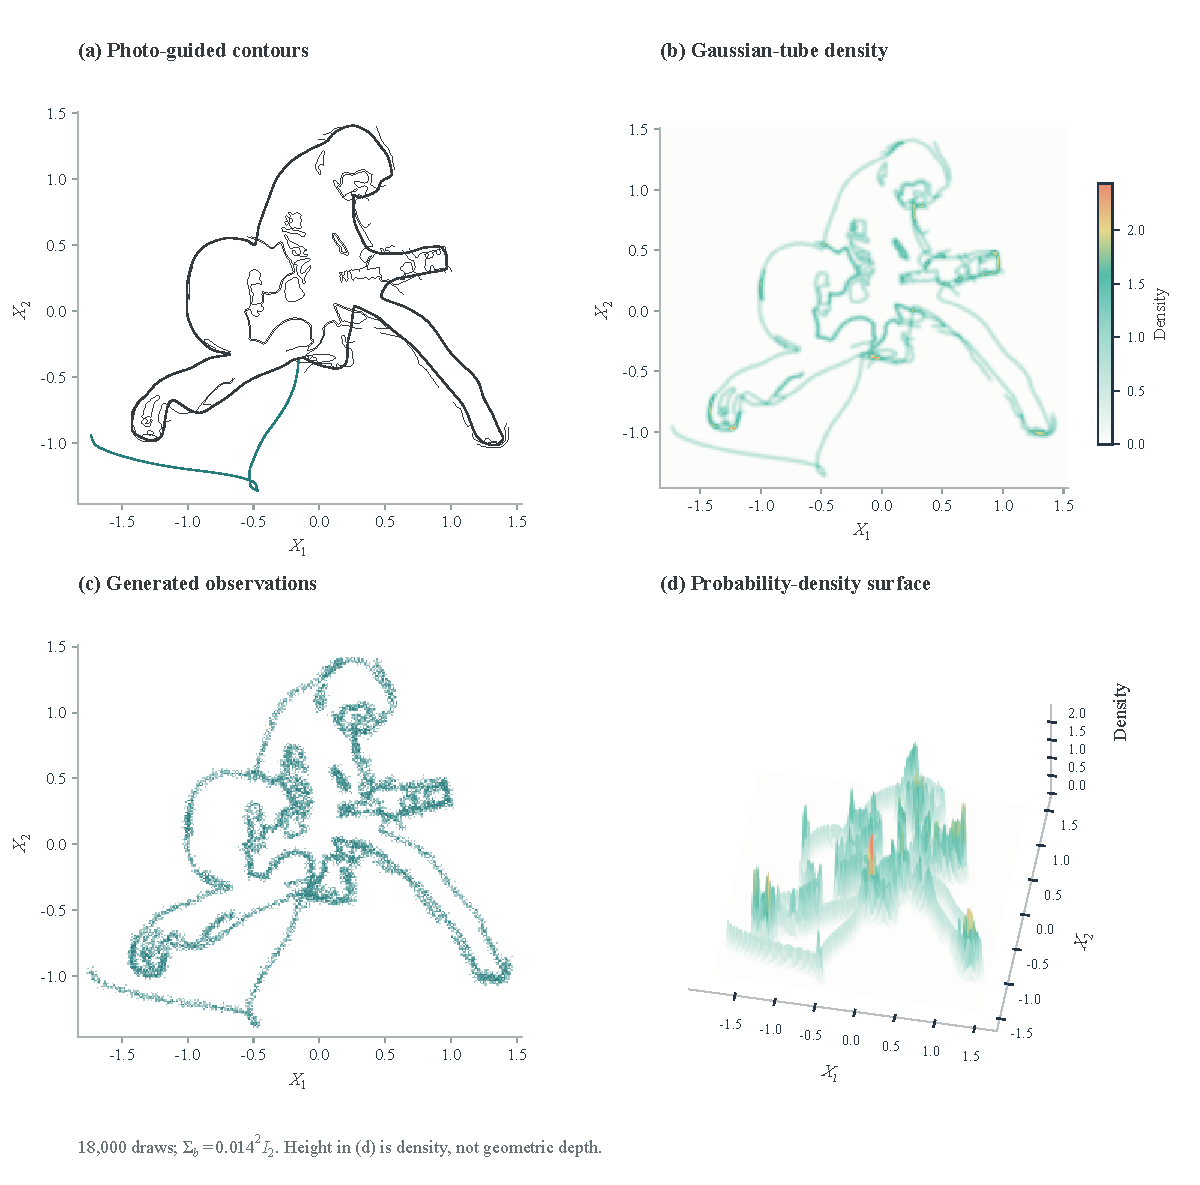
\includegraphics[width=0.97\linewidth,clip]{figures/elvis_sfd_four_panel.pdf}
\caption{An Elvis pose as a 35-component SFD. (a) Photo-guided curves,
with the cable in teal. (b) Gaussian-tube density with arclength weights
and covariance $0.014^2I_2$. (c) 18,000 generated observations.
(d) The same density as a surface: height represents density, not depth.}
\label{fig:elvis-example}
\end{figure}

For a fixed finite skeleton, a common dominating measure $\nu$ can include
Lebesgue measure, atom measures, and coordinate-pushforward measures of exact
branches. Densities in $p_\theta=dP_\theta/d\nu$ must all use that common
reference. If every component is regularized, Lebesgue measure suffices.
The experiments below use full-rank densities in common observed coordinates;
the mixed-measure formulation also covers exact strata. A moving singular
support requires a separate common-reference argument.

\begin{proposition}[Master expectation identity]
\label{prop:expectation}
For measurable $g$ with $\E_\theta|g(X)|<\infty$,
\begin{equation}
\begin{split}
\E_\theta g(X)
&=\sum_a\pi_a g(\xi_a)
 +\sum_b\pi_b\int_{\mathcal S_b}h_b(s)
                      \int g(x)K_b(dx\mid s)\,ds\\
&\quad+\sum_r\pi_r\int g(x)q_r(x)\,dx.
\end{split}
\label{eq:expectation}
\end{equation}
\end{proposition}
Condition on the component and then its coordinate to obtain the identity;
Tonelli--Fubini gives its integrable signed form. Appendix~\ref{app:calculus}
gives normalization, moments, mixed densities, marginals and conditionals.

\paragraph{Three distinct summaries.}
With component label $Z$ and branch coordinate $S$, the mass and longitudinal
mean are
\[
 \pi_b=\Pbb(Z=b),\qquad
 \bar s_b=\E(S\mid Z=b)=\int_{\mathcal S_b}s h_b(s)\,ds.
\]
The transverse part of the observation kernel describes spread around the
branch. These are latent-component quantities: overlapping tubes and
residuals also contribute probability to any observed neighborhood of a
curve. Consequently, that neighborhood probability generally differs from
$\pi_b$. Figure~\ref{fig:elvis-example} turns selected image-plane curves
into a concrete SFD by declaring their masses, coordinate laws and kernels.

\paragraph{Local geometry and coordinate conventions.}
For a regular curve, let $t_b(s)\in\R^d$ be its unit tangent and
$N_b(s)\in\R^{d\times(d-1)}$ an orthonormal normal frame. Independent
centered Gaussian perturbations along and normal to the curve give
\begin{equation}
 \begin{split}
 X&=\gamma_b(S)+t_b(S)\varepsilon_{\parallel,b}
                      +N_b(S)\varepsilon_{\perp,b},\\
 \Sigma_b(s)&=\sigma_{\parallel,b}^2(s)t_b(s)t_b(s)^\top
                +N_b(s)\Sigma_{\perp,b}(s)N_b(s)^\top.
 \end{split}
 \label{eq:frame}
\end{equation}
For a one-to-one regular $C^1$ exact branch with image $\Gamma_b$, the
conditional law $P_b=(\gamma_b)_\#\{h_b(s)ds\}$ has arc-length density
\begin{equation}
 \frac{dP_b}{d(\mathcal H^1|_{\Gamma_b})}\{\gamma_b(s)\}
       =\frac{h_b(s)}{\|\dot\gamma_b(s)\|}.
 \label{eq:intrinsic}
\end{equation}
Transporting the coordinate density and kernel under an increasing smooth
reparameterization preserves the branch law and mass. Coordinate means
require a common chart; normalized arc length removes coordinate warping
when origin, orientation, and branch correspondence are shared. Appendix~
\ref{app:geometry} gives the transformations and distinguishes latent
skeleton connectivity from the support of noisy observations.

\paragraph{Allocation and conditioning.}
For regularized component densities $g_c$,
\begin{equation}
 \Pbb(Z=c\mid X=x)=\frac{\pi_cg_c(x)}{\sum_{c'}\pi_{c'}g_{c'}(x)}.
 \label{eq:responsibility}
\end{equation}
For an event $A$ of positive probability, its component masses become
$\pi_cP_c(A)/\sum_{c'}\pi_{c'}P_{c'}(A)$. Marginals, event probabilities,
and conditional simulation follow from the same mixture law. The fitted
occupancy describes a static distribution; a model for time-ordered
observations is needed to estimate transition rates or probability flux.

\begin{proposition}[Single-trajectory tube special case]
\label{prop:single-tube}
Setting $\mathcal A=\mathcal R=\emptyset$, $\mathcal B=\{1\}$,
$\pi_1=1$ and
$K_1(dx\mid s)=\Normal(dx;\gamma_1(s),\Sigma_1(s))$ with positive-definite
$\Sigma_1(s)$ gives exactly
\[
 p_{\mathrm{tube}}(x)=\int_{\mathcal S_1}h_1(s)
       \phi_d\{x;\gamma_1(s),\Sigma_1(s)\}\,ds,
\]
where $\phi_d$ denotes the $d$-dimensional Gaussian density.
\end{proposition}
This follows by substitution in Definition~\ref{def:sfd}.
Appendix~\ref{app:special-cases} gives the other layer restrictions.

\paragraph{A circular branch and a volcano-shaped density.}
Take $\gamma(s)=1.2(\cos 2\pi s,\sin 2\pi s)$, uniform $S\in[0,1]$,
kernel covariance $0.16^2I_2$ and branch mass $0.94$. A centered Gaussian
residual has mass $0.06$ and covariance $1.25^2I_2$. The resulting
Lebesgue density concentrates around the ring while its centerline carries
zero observation probability. Figure~\ref{fig:volcano} displays the density,
an empirical histogram and the radial law. The construction separates a
branch's geometric image from its probability mass and observation width.

\begin{figure}[t]
\centering
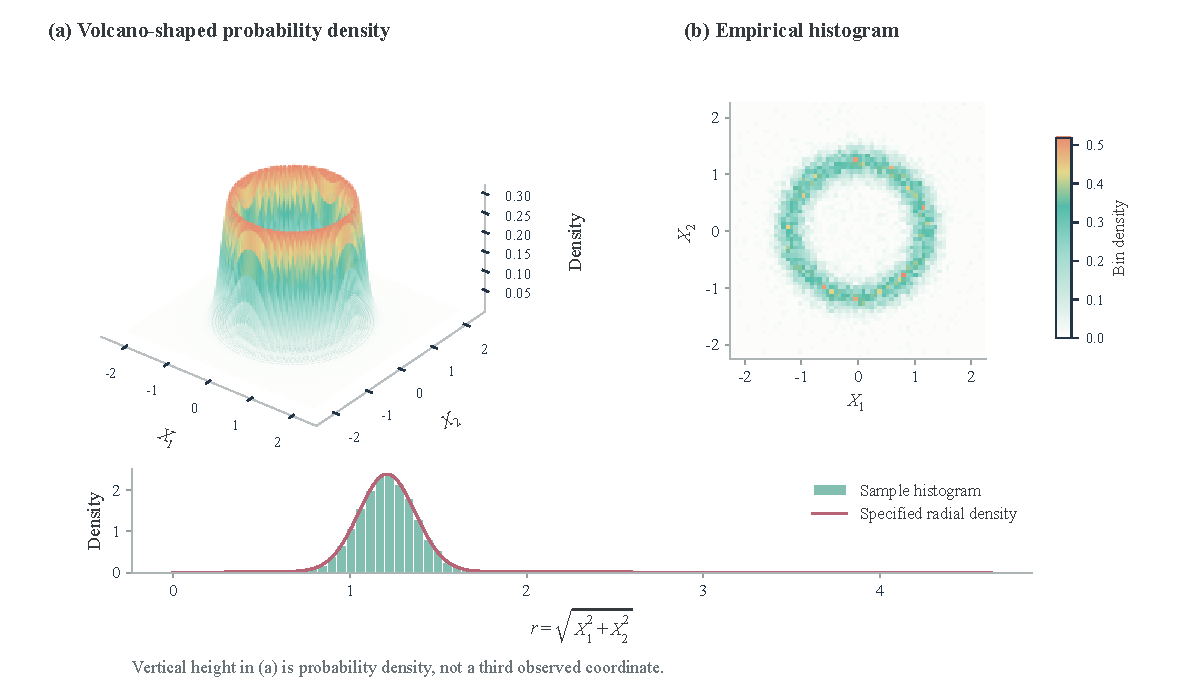
\includegraphics[width=0.97\linewidth,clip]{figures/volcano_density.pdf}
\caption{A circular Gaussian tube produces a volcano-shaped density.
(a) The specified density. (b) A bivariate histogram of 16,000 draws,
normalized by the full sample size. Bottom: sampled radii and their
density $2\pi r p(r)$.}
\label{fig:volcano}
\end{figure}
\paragraph{Projected geometry and reference samples.}
Figure~\ref{fig:fermat-section} uses a curved section of the Fermat quintic,
a Calabi--Yau hypersurface \citep{hendi2024invariant}. The section is
projected to $\R^3$ and approximated by 325 Gaussian tubes with equal masses
and covariance $0.035^2I_3$. The projection and coordinate-grid law are given
in Appendix~\ref{app:fermat-construction}. This example has three observed
coordinates, unlike the density heights in Figures~\ref{fig:elvis-example}d
and~\ref{fig:volcano}a.

\begin{figure}[t]
\centering
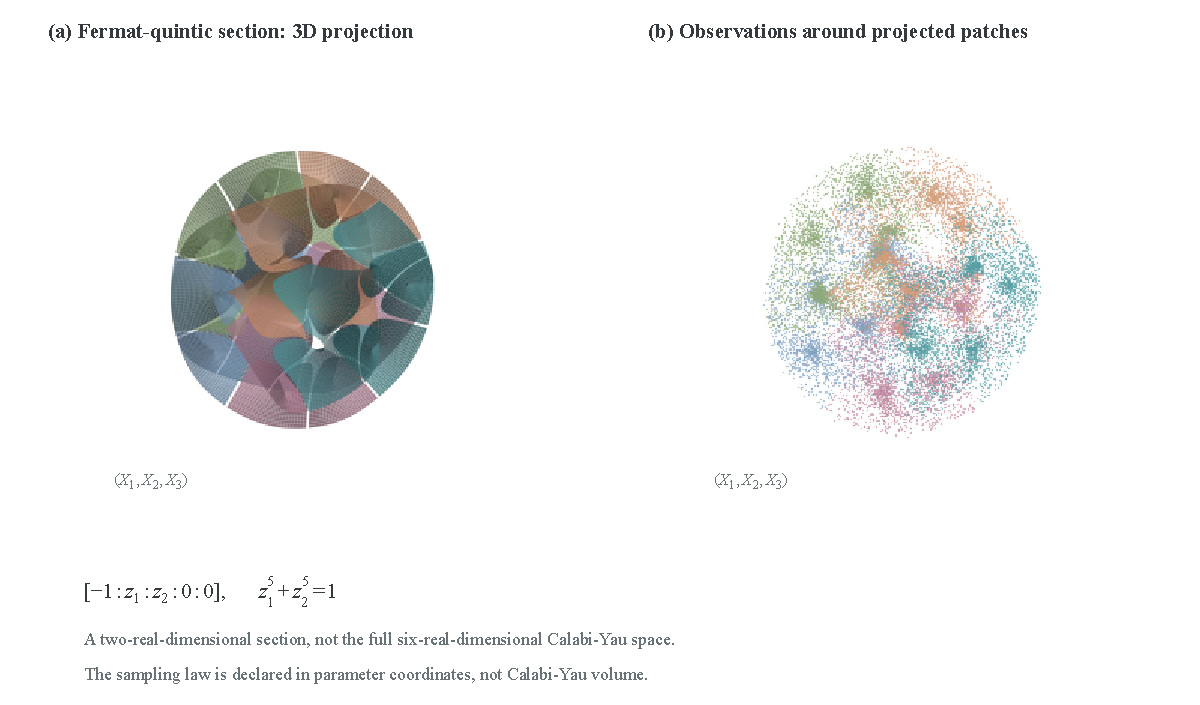
\includegraphics[width=0.97\linewidth,clip]{figures/fermat_section.pdf}
\caption{A projected Fermat-quintic section and an SFD around it. Left:
the geometric patches, colored by root index. Right: 18,000 observations
from 325 Gaussian tubes. Both panels use three spatial coordinates.}
\label{fig:fermat-section}
\end{figure}

Figure~\ref{fig:reference-histograms} complements these declared-geometry
examples with empirical views of Gaussian, skew-mixture and banana-transform
reference samples. Joint and marginal histograms expose different aspects
of the same sample shape. Each display uses 500 stored training observations;
the fitted-method comparisons begin in Section~\ref{sec:experiments}.
Appendix~\ref{app:visual-examples} records the construction details for
Figures~\ref{fig:elvis-example}--\ref{fig:reference-histograms}.

\begin{figure}[t]
\centering
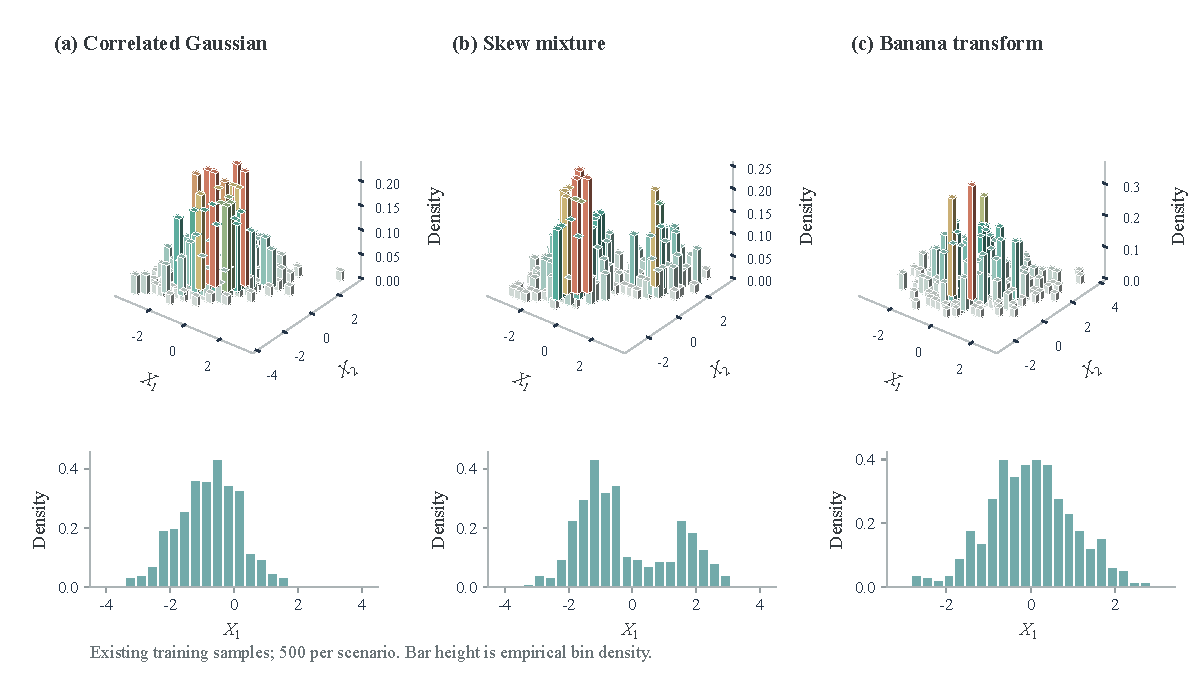
\includegraphics[width=0.97\linewidth,clip]{figures/reference_histograms.pdf}
\caption{Reference-sample histograms for a correlated Gaussian, skew mixture
and banana transform. Top: $24\times24$ bin densities in the first two
coordinates. Bottom: first-coordinate marginals. Each scenario uses all
500 training draws.}
\label{fig:reference-histograms}
\end{figure}

\paragraph{Density surfaces.}
Figure~\ref{fig:density-examples} shows four specified bivariate laws,
including a Doraemon-style face. These are density surfaces over two
coordinates, not three-dimensional observation models. Appendix~
\ref{app:visual-examples} records the display transformation.

\begin{figure}[t]
\centering
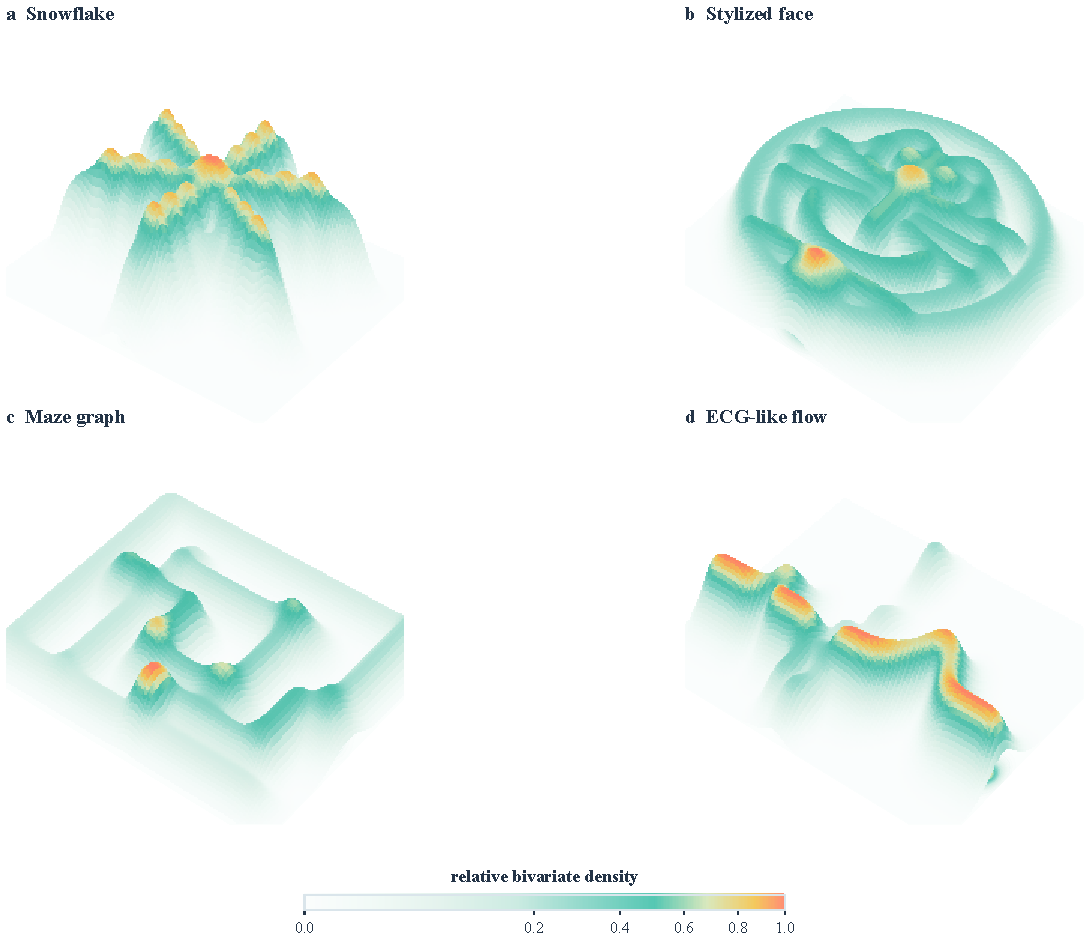
\includegraphics[width=0.94\linewidth,clip]{figures/specified_density_surfaces.pdf}
\caption{Specified snowflake, Doraemon-style face, maze and ECG-like
densities. Height and color use a separate nonlinear relative scale in each
panel, revealing shape rather than comparing absolute density. Curves
contribute Gaussian tubes; localized peaks are Gaussian blobs.}
\label{fig:density-examples}
\end{figure}

\FloatBarrier

\section{Normalized Finite-Skeleton Estimation}
\label{sec:learning}
Positive quadrature weights $w_{bm}$ and coordinate nodes $s_{bm}$ give
\begin{equation}
 C_b(\eta_b)=\sum_mw_{bm}h_b(s_{bm};\eta_b),\qquad
 \kappa_{bm}(\eta_b)=\frac{w_{bm}h_b(s_{bm};\eta_b)}{C_b(\eta_b)},\qquad
 g_b^{\mathrm{grid}}(x)=\sum_m\kappa_{bm}k_b(x\mid s_{bm}).
 \label{eq:grid}
\end{equation}
For $C_b>0$, the node probabilities sum to one and each finite-grid branch
is normalized. Normalization is essential when $h_b$ changes: otherwise its
quadrature error can enter the apparent branch mass. Accuracy relative to
the continuous integral remains a grid-resolution question.

The declared objective is
\begin{equation}
 F_n(\theta)=\sum_i\log p_\theta^{\mathrm{grid}}(x_i)
                  -\operatorname{Pen}(\theta).
 \label{eq:objective}
\end{equation}
Node responsibilities are
$r_{ibm}=\pi_b\kappa_{bm}k_b(x_i\mid s_{bm})/p_\theta^{\mathrm{grid}}(x_i)$.
Writing $n_b^{\mathrm{eff}}=\sum_{i,m}r_{ibm}$, the occupancy block of the
EM surrogate contains
\begin{equation}
 \sum_{i,m}r_{ibm}\log h_b(s_{bm};\eta_b)
                 -n_b^{\mathrm{eff}}\log C_b(\eta_b).
 \label{eq:occupancy}
\end{equation}
Its second term must remain in the optimization. A Dirichlet penalty on
outer masses yields updates proportional to $n_c^{\mathrm{eff}}+\alpha_c-1$
when $\alpha_c>1$; penalties on other parameters remain in their respective
blocks.

\begin{algorithm}[H]
\caption{Objective-checked finite-grid estimation}
\label{alg:grid}
\begin{algorithmic}[1]
\Require Observations, declared branches and component families, positive
quadrature rule, penalty, feasible starts, and stopping tolerances.
\For{each start}
 \State Normalize node probabilities $\kappa_{bm}$ and evaluate $F_n$.
 \Repeat
  \State Compute responsibilities for all nodes and residual components.
  \State Update masses and propose occupancy, geometry, and noise blocks.
  \State Retain the normalizer in \eqref{eq:occupancy} and all penalties.
  \State Accept feasible block steps only if they do not decrease $F_n$.
 \Until{objective and stationarity tolerances hold, or the iteration limit is reached}
 \State Record the objective, stopping status, and any active constraints.
\EndFor
\State Select the feasible fit with largest recorded objective; retain all statuses.
\end{algorithmic}
\end{algorithm}

\begin{proposition}[Fixed-quadrature GEM monotonicity]
\label{prop:gem}
Fix the normalized quadrature law, latent label set, parameter space and
penalty. Suppose the observed densities are finite and positive at the old
and proposed iterates. An update that does not decrease the penalized
expected complete-data objective cannot decrease $F_n$.
\end{proposition}
The proof is the EM lower-bound argument
\citep{dempster1977em,wu1983convergence}, given in
Appendix~\ref{app:numerical-theory}. Algorithm~\ref{alg:grid}
states the objective checks for approximate block updates. After covariance
factorization, a responsibility pass costs $O(nMd^2)$ for $M$ dense-covariance
nodes, or $O(nMd)$ for isotropic kernels. This per-pass calculation leaves the
number of iterations and nonconvex optimization behavior to the selected
parameterization.

With fixed kernels, weight estimation is concave. A positive pseudocount
penalty can select a unique maximizer even when some likelihood weights are
unidentified. The next section distinguishes optimization uniqueness from
identification. The two-arm experiments use closed-form longitudinal
convolution and direct likelihood optimization. The PBMC analysis uses a
specified MST width/residual heuristic; its small-mass-change stopping rule
is reported separately from objective-checked GEM.

\section{Identification and Fixed-Stratum Inference}
\label{sec:identification}
\subsection{Identification of a Grouped Mass}
Fix normalized kernels $f_1,\ldots,f_K$ relative to $\nu$, their grouping,
and an interior simplex weight $w\in\R^K$. Write $p_w=\sum_jw_jf_j$ and
$T_\zeta(w)=\zeta^\top w$. For a branch mass, $\zeta$ indicates the nodes
assigned to that branch. Define the likelihood-null directions
\begin{equation}
 \mathcal V_0=\{v\in\R^K:\ \boldsymbol 1^\top v=0,
                  \textstyle\sum_jv_jf_j=0\ \nu\text{-a.e.}\}.
 \label{eq:nullspace}
\end{equation}
\begin{proposition}[Fixed-kernel grouped target]
\label{prop:identification}
The target $T_\zeta$ is identified on the interior simplex exactly when
$\zeta\perp\mathcal V_0$. Eliminate $w_K$ and set, for $j<K$,
\begin{equation}
 U_j(x)=\frac{f_j(x)-f_K(x)}{p_w(x)},\qquad
 I_w=\E_w\{U(X)U(X)^\top\},\qquad
 \beta_{\zeta,j}=\zeta_j-\zeta_K,
 \label{eq:information}
\end{equation}
with $U=0$ where $p_w=0$. Identification is equivalent to
$\beta_\zeta\in\operatorname{range}(I_w)$. Every centered square-integrable
influence function $\phi$ satisfying $\E_w(\phi U)=\beta_\zeta$ obeys
\begin{equation}
\E_w(\phi^2)\ge\beta_\zeta^\top I_w^+\beta_\zeta,
 \label{eq:bound}
\end{equation}
where $I_w^+$ is the Moore-Penrose pseudoinverse.
\end{proposition}

Equal mixture densities have weight difference in $\mathcal V_0$.
Orthogonality therefore gives sufficiency, and a small interior perturbation
along a null direction gives necessity. The null space of $I_w$ describes
the same density-preserving directions; projection onto the score span gives
the bound. Appendix~\ref{app:proof} supplies the proof. The result applies
standard mixture-identification and information arguments
\citep{mclachlan2000finite,vandervaart1998asymptotic} to the declared grouped
target.

If $f_1=f_2$ within one branch, their separate weights are unidentified but
their sum can remain identified when the branch separates from the other
kernels. Assigning those duplicate kernels to different branches instead
destroys identification of the separate masses. Refining a within-branch
grid and increasing cross-branch overlap can therefore have different
consequences for the same target.

This information bound conditions on fixed kernels. Estimating noise,
geometry, residuals, or the grouping introduces additional nuisance
directions. Prior curvature can select among observationally equivalent
weights but cannot identify them from the likelihood. For fitted six- and
eight-parameter two-arm models, Section~\ref{sec:intervals} instead evaluates
intervals using the complete estimated parameter chart.

\subsection{Regular Fixed-Stratum Likelihood Theory}
Joint estimation follows regular likelihood theory on an identifiable
fixed-stratum chart \citep{vandervaart1998asymptotic}.

\begin{theorem}[Regular finite-SFD likelihood theory]
\label{thm:regular-finite-sfd}
Let $X_i\stackrel{\mathrm{iid}}\sim P_{\theta_0}$ in a finite SFD chart
satisfying conditions \textup{(R1)--(R5)} of
Appendix~\ref{app:regular-conditions}. Put
$U_0=\nabla\log p_{\theta_0}$ and
$I_0=\E_{\theta_0}(U_0U_0^\top)\succ0$.
The consistent interior likelihood maximizer $\hat\theta_n$ satisfies
\begin{equation}
 \sqrt n(\hat\theta_n-\theta_0)
 =I_0^{-1}n^{-1/2}\sum_i U_0(X_i)+o_p(1)
 \ \rightsquigarrow\ \Normal(0,I_0^{-1}).
 \label{eq:regular-limit}
\end{equation}
For every differentiable fixed-stratum target $\psi$,
\begin{equation}
 \sqrt n\{\psi(\hat\theta_n)-\psi(\theta_0)\}
 \ \rightsquigarrow\ \Normal\!\left(0,
 \dot\psi(\theta_0)I_0^{-1}\dot\psi(\theta_0)^\top\right).
 \label{eq:target-limit}
\end{equation}
\end{theorem}
The proof and regular contrast tests are in Appendix~\ref{app:regular-theory};
Appendix~\ref{app:numerical-theory} treats numerical-likelihood transfer.

\clearpage
\section{Experiments}
\label{sec:experiments}
Four studies assess weight estimation on a supplied skeleton, target recovery,
sensitivity to geometry and noise, and allocation as a prediction feature.
Each uses 25 repetitions. Simulation
repetitions are independent; PBMC splits overlap within one cell collection.
Numbers in parentheses are Monte Carlo SEs of displayed means. Generating
labels are used for evaluation, not fitting. Appendix~\ref{app:experiments}
specifies optimizers, controls, preprocessing, and stopping rules; all
prespecified density and marker controls appear in Appendix~\ref{app:controls}.

\subsection{Known-Skeleton Weight Estimation}
\label{sec:known-skeleton}
Five specified laws use snowflake, stylized-face, maze, ECG-like, and
torus-knot geometries. Each repetition provides 1000 training observations
and 1000 independent test observations. EM estimates the component masses
with the generating geometry, coordinate laws and noise kernels fixed;
each tube integral uses 64 coordinate nodes. Figure~\ref{fig:known-skeleton-fitted}
shows test log density, component-mass RMSE and component-label accuracy.
The oracle evaluates the generating law, rather than an estimated model.
This diagnostic isolates mass estimation from geometry and noise estimation;
the next two studies examine the latter distinction. Appendix~
\ref{app:external-density-controls} gives classical-distribution and copula
reference controls separately.

\begin{figure}[H]
\centering
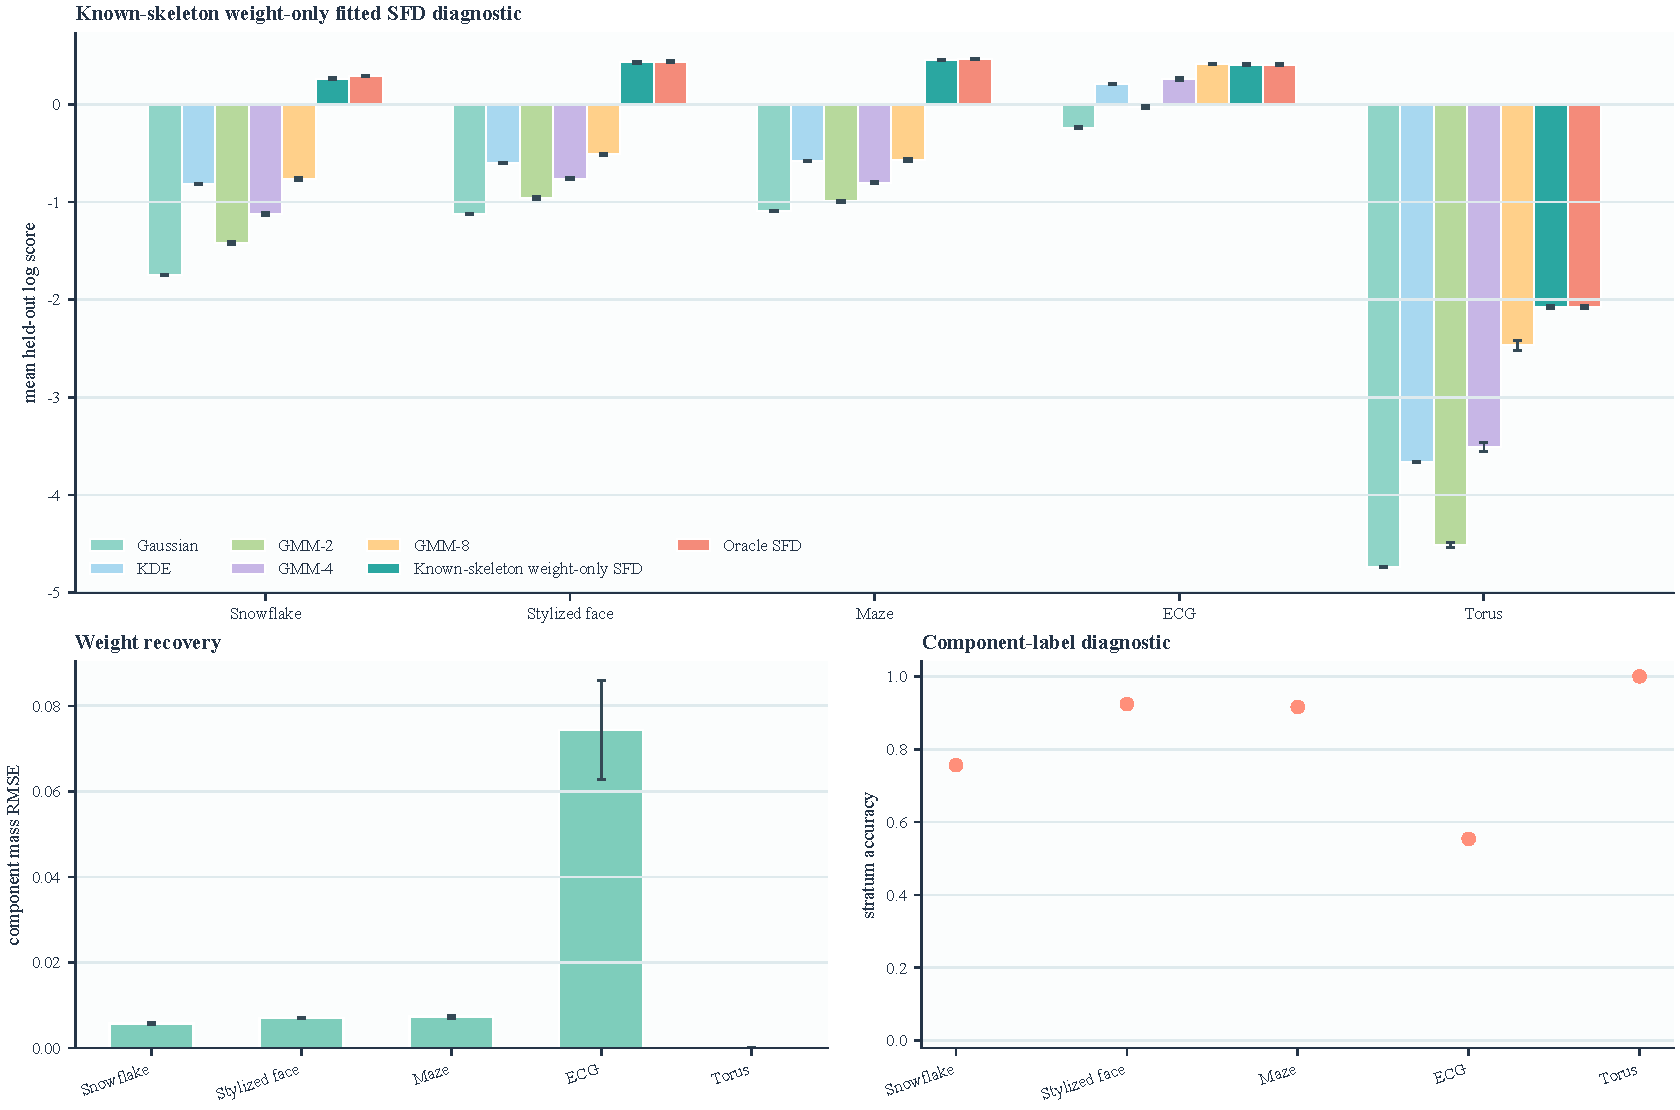
\includegraphics[width=\linewidth,clip]{figures/known_skeleton_fitted.pdf}
\caption{Weight-only SFD fitting on five supplied skeletons. Top: test log
density for generic controls, fitted SFD and the oracle. Bottom: fitted
component-mass RMSE and component-label accuracy. Bars show one Monte Carlo
SE over 25 repetitions. The generating geometry and kernels are fixed;
truth labels are used only for evaluation. GMM-16 and GMM-32 results are
retained in the accompanying summary data.}
\label{fig:known-skeleton-fitted}
\end{figure}
\FloatBarrier

\subsection{When a Width Change Becomes a Mass Change}
Two unit-length arms meet at angles $\pm\pi/6$. Each branch coordinate is
$\Normal(\mu_b^{\mathrm{loc}},0.16^2)$ truncated to $[0,1]$. Observation
noise has tangent SD $0.025$ and normal SD $\sigma_b$. The residual is
$\Normal((0.4,0),0.55^2 I_2)$. The reference has masses $(0.4,0.4,0.2)$,
locations $(0.5,0.5)$, and widths $(0.07,0.07)$. Three alternatives change
only masses to $(0.6,0.2,0.2)$, the upper location to $0.7$, or the upper
width to $0.14$. Each group supplies 1000 training and 2000 independent test
observations per repetition. The location parameter and truncated coordinate
mean are distinct; the position alternative changes the latter by about
$0.189$.

The joint fit estimates two mass logits, two occupancy locations, and two
normal widths, with origin, directions, coordinate scale, tangent noise,
and residual law supplied. Two mass-only ablations fix either the reference
kernels or the true group-specific kernels. This comparison isolates the
consequence of fixing a kernel that changes between groups.

\begin{figure}[t]
\centering
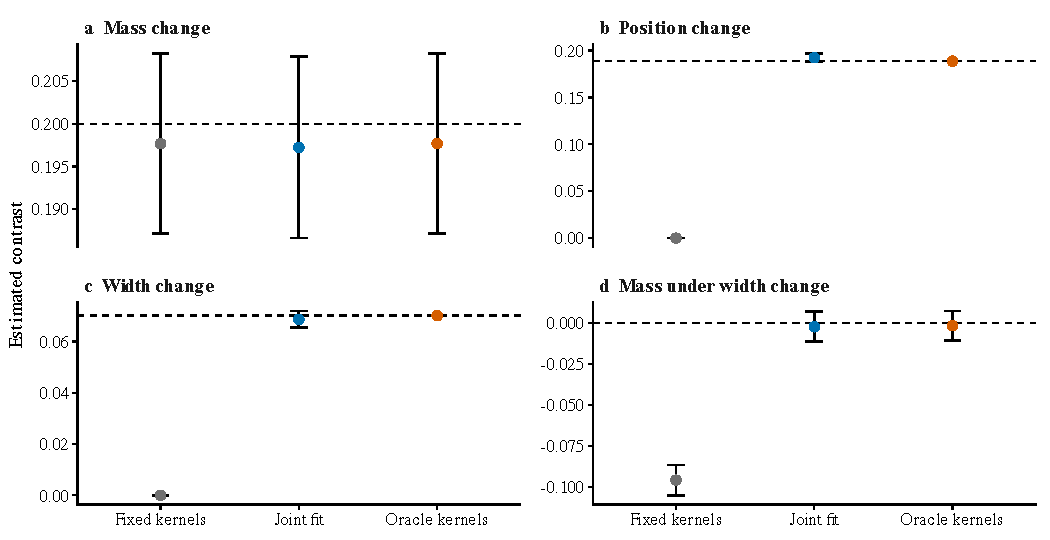
\includegraphics[width=\linewidth,clip]{figures/mechanism_separation.pdf}
\caption{Two-arm target recovery. Panels a--c show mass, coordinate-mean
and width contrasts; d shows the mass contrast under a width-only change.
Dashed lines mark truth. Points and bars give means and $\pm1.96$ Monte
Carlo SEs over 25 repetitions. The two kernel ablations estimate masses only.}
\label{fig:mechanism}
\end{figure}

The joint estimates are \MechMass{} for the mass contrast, \MechPosition{}
for position, and \MechWidth{} for width, against generating contrasts
$0.200$, $0.189$, and $0.0700$. Under the width-only alternative the true
mass contrast is zero, yet fixed reference kernels produce
\MechFixedSpurious{}. Joint estimation produces \MechJointSpurious{}
(Figure~\ref{fig:mechanism}). The fixed-width model explains some increased
transverse spread by lowering the fitted branch mass. All 300 selected SFD
fits meet their optimizer stopping rule without parameter-bound contacts.

Gaussian, GMM-4, GMM-8, and KDE controls are scored on test log density and
the observable probability $\Pbb(X_2>0)$. Their components are not assigned
branch labels. These controls assess prediction, whereas the joint-versus-
fixed comparison assesses kernel constraints on a specified latent target.
Every run, including GMM iteration-limit warnings, is retained in the
supplementary score tables.

\subsection{Estimated Directions and Misspecified Noise}
The four group laws are repeated with Gaussian arms at $\pm30^\circ$,
overlapping arms at $\pm15^\circ$, and $\pm30^\circ$ arms with transverse
Student-$t_5$ noise scaled to the same SD. Each condition has the same sample
sizes and 25 repetitions. Fits use correct directions, rotate both by
$5^\circ$, or estimate two angles from training coordinates. The
learned-direction fit has eight parameters and retains the supplied origin,
two-arm family, coordinate and tangent scales, and residual law.

\begin{figure}[t]
\centering
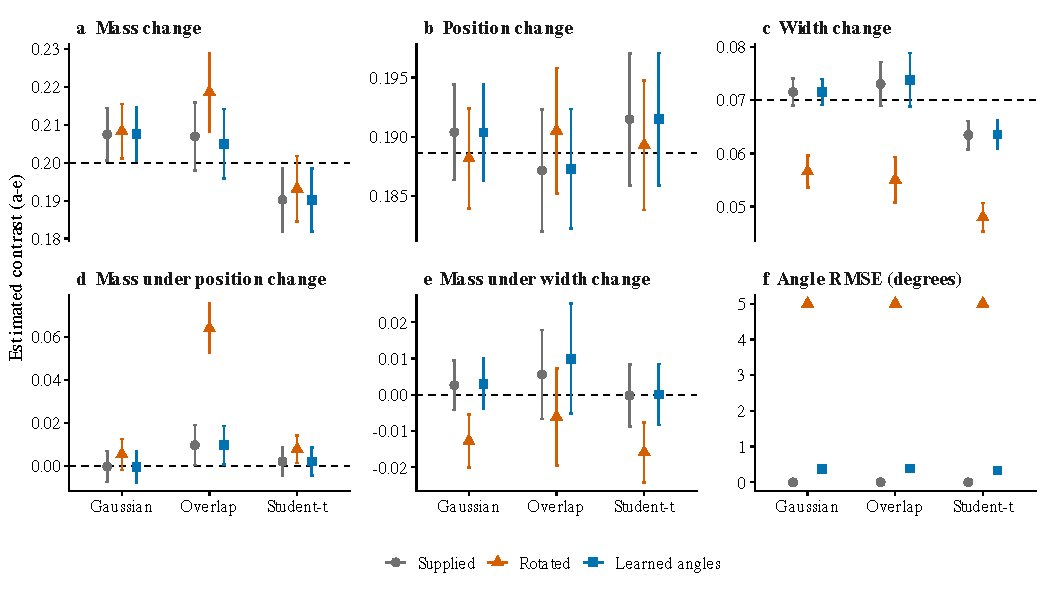
\includegraphics[width=\linewidth,clip]{figures/geometry_validation.pdf}
\caption{Geometry and noise sensitivity under supplied, $5^\circ$-rotated
or learned directions. Panels a--e show target contrasts and mass
cross-effects; f shows angle RMSE in degrees. Dashed lines mark truth;
bars give $\pm1.96$ Monte Carlo SEs over 25 repetitions. All fitted tubes
are Gaussian, including those fitted to Student-$t_5$ noise.}
\label{fig:geometry}
\end{figure}

The learned-angle reference RMSEs are \AngleGaussian{}, \AngleOverlap{},
and \AngleHeavy{} degrees. Estimated width contrasts are \WidthGaussian{},
\WidthOverlap{}, and \WidthHeavy{}, against $0.0700$. Under heavy-tailed
noise, learning directions leaves a systematic width discrepancy under the
Gaussian fitted family. Figure~\ref{fig:geometry} also shows the effects of
overlap and direction error on mass contrasts. All 900 selected SFD fits
meet their stopping rule without boundary contacts; selected GMM fits
converge under the expanded budget.

\paragraph{Parameter intervals.}
\label{sec:intervals}
A post-hoc calculation uses each saved fit's complete six- or eight-parameter
information matrix, including angles when estimated. With learned directions
and Gaussian noise, nominal 95\% Wald intervals cover generating mass,
position, and width contrasts in \CovGaussianLearnedMass{},
\CovGaussianLearnedPosition{}, and \CovGaussianLearnedWidth{} repetitions.
For rotated directions with Student-$t_5$ noise, width-contrast coverage is
\CovHeavyRotatedInfo{} with information covariance and
\CovHeavyRotatedSand{} with sandwich covariance. The latter adjusts
estimated variability, not misspecification of the fitted center. These
parameter intervals are distinct from the Monte Carlo bars in
Figure~\ref{fig:geometry}. Appendix~\ref{app:intervals} reports the full
calculation, numerical checks, and coverage counts. Each count has only
25 repetitions, so even 25/25 provides limited precision about coverage.

\FloatBarrier
\subsection{Allocation as a Feature-Held-Out Readout}
The public PBMC3k collection \citep{tenxgenomics2016pbmc3k} supplies an
internal prediction study. In each of 25 splits, 2160 cells train the
representation and 540 are held out. Eighteen predeclared marker genes are
excluded from predictor normalization and selection. Training cells alone
determine gene filtering, the 1000 selected nonmarker genes, scaling,
clipping, and two-component PCA. Test cells use those transforms. Density
scores refer to this two-dimensional representation, not the gene-count space.

An MST-skeleton tube with Gaussian residual is compared with Gaussian, GMM,
and KDE densities. Mean test log density is \PBMCDensitySFD{} for SFD,
\PBMCDensityGMM{} for GMM-8, and \PBMCDensityKDE{} for KDE; generic controls
give the stronger density predictions here (Figure~\ref{fig:pbmc}). The
allocation question is whether a posterior tube feature adds information
beyond the two PCs and KDE log density.

\begin{figure}[t]
\centering
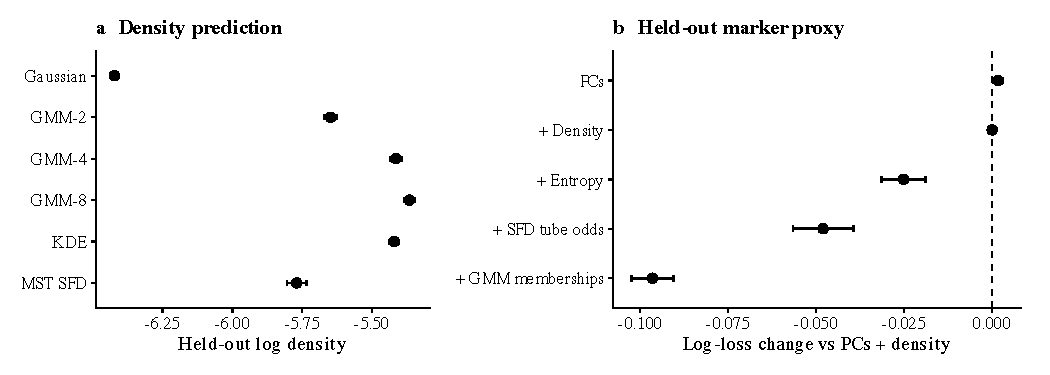
\includegraphics[width=\linewidth,clip]{figures/pbmc_inductive_validation.pdf}
\caption{PBMC readouts on training-fitted PCs. a: test log density.
b: paired log-loss changes for the held-out B-marker proxy, relative to
PCs plus KDE density. SFD adds one tube-odds feature; GMM adds seven
memberships. Bars give $\pm1.96$ split Monte Carlo SEs over 25 overlapping
cell splits, not donor-level uncertainty.}
\label{fig:pbmc}
\end{figure}

The binary outcome is a predeclared B-marker proxy computed from the held-out
marker panel. Logistic readouts share the inner validation cells and penalty
grid. Adding scalar SFD tube log odds changes mean test log loss from
\PBMCMarkerBase{} to \PBMCMarkerSFD{}, a paired difference of
\PBMCPairedSFD{}. GMM posterior entropy gives \PBMCMarkerEntropy{};
seven GMM membership coordinates give \PBMCMarkerMembership{}. Allocation
features therefore improve this readout beyond density features, with the
larger generic-mixture representation performing better. These unequal-
dimension readouts predict a marker proxy within one collection; they do
not estimate independent-donor uncertainty.
\FloatBarrier

\section{Discussion}
SFD separates branch probability, longitudinal occupancy, and observation
noise within one declared probability law. The two-arm experiments show why
this separation matters: a fixed-width constraint can turn increased spread
into an apparent mass decrease, and estimating both blocks corrects that
error under the specified model. The identification analysis explains why
grouped masses can remain meaningful when numerical subdivisions are
unidentified, and where overlap prevents that interpretation.

The interpretation conditions on a declared skeleton and kernel family.
The experiments supply a two-arm family or a particular MST representation;
arbitrary topology recovery is a separate problem. PBMC shows allocation
features within a training-fitted representation, with stronger generic
controls retained. Scientific state interpretation requires independently
defined states and sampling units. A prospective time-resolved model would
add a latent stochastic process and temporal observations
(Appendix~\ref{app:geometry}).

\clearpage
\section*{Code and Data Availability}
The software, experiment scripts, saved per-repetition results, and manuscript
sources are available at
\begin{center}
\url{https://github.com/ElvisCuiHan/stratified-flow-distributions}
\end{center}
The repository includes instructions for checking numerical summaries,
regenerating figures, and rerunning experiments. PBMC3k raw data are available
from 10x Genomics \citep{tenxgenomics2016pbmc3k}; preprocessing and analysis
settings are given in Appendix~\ref{app:experiments}.

Figure~\ref{fig:elvis-example} reconstructs a pose
from an author-supplied Elvis Presley photograph; the photograph itself is
not reproduced. Figures~\ref{fig:density-examples}b and
\ref{fig:face-example} use a Doraemon-inspired synthetic geometry.

\section*{License}
The author-authored text and original scientific material are licensed under
Creative Commons Attribution 4.0 International. This license excludes
third-party rights in the Elvis-derived illustration and Doraemon-inspired
examples. Their inclusion does not grant permission to reuse those elements.
Document styles retain their own license notices in the compilation archive.
The original software is released separately under the MIT license.
\label{maintext:end}
\clearpage
\begin{thebibliography}{99}
\bibitem[10x Genomics(2016)]{tenxgenomics2016pbmc3k}
10x Genomics (2016).
3k PBMCs from a healthy donor.
\emph{10x Genomics datasets}.
\url{https://www.10xgenomics.com/datasets/3-k-pbm-cs-from-a-healthy-donor-1-standard-1-1-0}.
Accessed 25 June 2026.

\bibitem[Arvanitidis et~al.(2016)]{arvanitidis2016land}
Arvanitidis, G., Hansen, L. K., and Hauberg, S. (2016).
A locally adaptive normal distribution.
\emph{Advances in Neural Information Processing Systems}, 29.

\bibitem[Billera et~al.(2001)]{billera2001geometry}
Billera, L. J., Holmes, S. P., and Vogtmann, K. (2001).
Geometry of the space of phylogenetic trees.
\emph{Advances in Applied Mathematics}, 27(4), 733--767.

\bibitem[Bishop et~al.(1998)]{bishop1998gtm}
Bishop, C. M., Svensen, M., and Williams, C. K. I. (1998).
GTM: The generative topographic mapping.
\emph{Neural Computation}, 10(1), 215--234.

\bibitem[Boucheron et~al.(2013)]{boucheron2013concentration}
Boucheron, S., Lugosi, G., and Massart, P. (2013).
\emph{Concentration Inequalities: A Nonasymptotic Theory of Independence}.
Oxford University Press.

\bibitem[Coifman and Lafon(2006)]{coifman2006diffusion}
Coifman, R. R. and Lafon, S. (2006).
Diffusion maps.
\emph{Applied and Computational Harmonic Analysis}, 21(1), 5--30.

\bibitem[Dempster et~al.(1977)]{dempster1977em}
Dempster, A. P., Laird, N. M., and Rubin, D. B. (1977).
Maximum likelihood from incomplete data via the EM algorithm.
\emph{Journal of the Royal Statistical Society: Series B}, 39(1), 1--38.

\bibitem[Genovese et~al.(2012)]{genovese2012manifold}
Genovese, C. R., Perone-Pacifico, M., Verdinelli, I., and Wasserman, L. (2012).
Manifold estimation and singular deconvolution under Hausdorff loss.
\emph{The Annals of Statistics}, 40(2), 941--963.

\bibitem[Hastie and Stuetzle(1989)]{hastie1989principal}
Hastie, T. and Stuetzle, W. (1989).
Principal curves.
\emph{Journal of the American Statistical Association}, 84(406), 502--516.

\bibitem[Hendi et~al.(2024)]{hendi2024invariant}
Hendi, Y., Larfors, M., and Walden, M. (2024).
Learning group invariant Calabi--Yau metrics by fundamental domain projections.
\emph{arXiv:2407.06914v2}.
\url{https://arxiv.org/abs/2407.06914}.

\bibitem[Hotz et~al.(2013)]{hotz2013sticky}
Hotz, T., Huckemann, S., Le, H., Marron, J. S., Mattingly, J. C.,
Miller, E., Nolen, J., Owen, M., Patrangenaru, V., and Skwerer, S. (2013).
Sticky central limit theorems on open books.
\emph{The Annals of Applied Probability}, 23(6), 2238--2258.

\bibitem[Kostrykin et~al.(2012)]{kostrykin2012brownian}
Kostrykin, V., Potthoff, J., and Schrader, R. (2012).
Brownian motions on metric graphs.
\emph{arXiv:1102.4937v3}.
\url{https://arxiv.org/abs/1102.4937}.

\bibitem[Lipman et~al.(2023)]{lipman2023flow}
Lipman, Y., Chen, R. T. Q., Ben-Hamu, H., Nickel, M., and Le, M. (2023).
Flow matching for generative modeling.
\emph{International Conference on Learning Representations}.

\bibitem[Mathieu and Nickel(2020)]{mathieu2020riemannian}
Mathieu, E. and Nickel, M. (2020).
Riemannian continuous normalizing flows.
\emph{Advances in Neural Information Processing Systems}, 33.

\bibitem[McLachlan and Peel(2000)]{mclachlan2000finite}
McLachlan, G. and Peel, D. (2000).
\emph{Finite Mixture Models}.
Wiley.

\bibitem[Nelsen(2006)]{nelsen2006copulas}
Nelsen, R. B. (2006).
\emph{An Introduction to Copulas}.
Second edition. Springer.

\bibitem[Papamakarios et~al.(2021)]{papamakarios2021normalizing}
Papamakarios, G., Nalisnick, E., Rezende, D. J., Mohamed, S., and
Lakshminarayanan, B. (2021).
Normalizing flows for probabilistic modeling and inference.
\emph{Journal of Machine Learning Research}, 22(57), 1--64.

\bibitem[Schiebinger et~al.(2019)]{schiebinger2019optimal}
Schiebinger, G., Shu, J., Tabaka, M., Cleary, B., Subramanian, V.,
Solomon, A., Gould, J., Liu, S., Lin, S., Berube, P., Lee, L., Chen, J.,
Brumbaugh, J., Rigollet, P., Hochedlinger, K., Jaenisch, R., Regev, A., and
Lander, E. S. (2019).
Optimal-transport analysis of single-cell gene expression identifies
developmental trajectories in reprogramming.
\emph{Cell}, 176(4), 928--943.e22.

\bibitem[Silverman(1986)]{silverman1986density}
Silverman, B. W. (1986).
\emph{Density Estimation for Statistics and Data Analysis}.
Chapman and Hall.

\bibitem[Song et~al.(2021)]{song2021score}
Song, Y., Sohl-Dickstein, J., Kingma, D. P., Kumar, A., Ermon, S., and
Poole, B. (2021).
Score-based generative modeling through stochastic differential equations.
\emph{International Conference on Learning Representations}.

\bibitem[Tenenbaum et~al.(2000)]{tenenbaum2000isomap}
Tenenbaum, J. B., de Silva, V., and Langford, J. C. (2000).
A global geometric framework for nonlinear dimensionality reduction.
\emph{Science}, 290(5500), 2319--2323.

\bibitem[Trapnell et~al.(2014)]{trapnell2014dynamics}
Trapnell, C., Cacchiarelli, D., Grimsby, J., Pokharel, P., Li, S., Morse, M.,
Lennon, N. J., Livak, K. J., Mikkelsen, T. S., and Rinn, J. L. (2014).
The dynamics and regulators of cell fate decisions are revealed by
pseudotemporal ordering of single cells.
\emph{Nature Biotechnology}, 32(4), 381--386.

\bibitem[van der Vaart(1998)]{vandervaart1998asymptotic}
van der Vaart, A. W. (1998).
\emph{Asymptotic Statistics}.
Cambridge University Press.

\bibitem[Wu(1983)]{wu1983convergence}
Wu, C. F. J. (1983).
On the convergence properties of the EM algorithm.
\emph{The Annals of Statistics}, 11(1), 95--103.
\end{thebibliography}

\clearpage
\appendix
\section{Fixed-Kernel Identification and Information}
\label{app:proof}
The result in Proposition~\ref{prop:identification} holds for arbitrary normalized
nonnegative kernels under a fixed reference measure, including mixed measures.
It is conditional on their scientific grouping and on an interior weight.

If $p_w=p_{w'}$, then $v=w-w'\in\mathcal V_0$. Orthogonality of $\zeta$ therefore
makes $T_\zeta(w)=T_\zeta(w')$. Conversely, if $\zeta^\top v\ne0$ for some
$v\in\mathcal V_0$, every interior $w$ admits a sufficiently small nonzero
$t$ such that $w+tv$ stays in the simplex interior. Its density is unchanged,
but its target changes by $t\zeta^\top v$. This proves both directions.

For positive $w$, $f_j/p_w\le 1/w_j$ on the density support. Each score
component in (\ref{eq:information}) is therefore square integrable. For
$a\in\R^{K-1}$, $a^\top I_wa=0$ exactly when
$\sum_{j<K}a_j(f_j-f_K)=0$ almost everywhere. Its corresponding full null
direction is $(a_1,\ldots,a_{K-1},-\sum_{j<K}a_j)$. The target annihilates this
null space exactly when $\beta_\zeta$ belongs to the range of $I_w$.
When it does, $\phi_* =\beta_\zeta^\top I_w^+U$ is centered and satisfies
$\E_w(\phi_*U)=\beta_\zeta$. Any other centered square-integrable $\phi$ with
the same covariance has $\phi-\phi_*$ orthogonal to the score span. Hence
$\E_w(\phi^2)=\E_w(\phi_*^2)+\E_w\{(\phi-\phi_*)^2\}$, giving the bound.
This is an influence-function variance bound, not a claim that a particular
adaptive estimator attains it. Its sample-mean asymptotic variance factor is
conditional on fixed kernels; nuisance estimation is not covered.

\paragraph{Penalized uniqueness and likelihood identification.}
For $\tau>0$ and every $r_j>0$, consider
\[
 L_n(w)=\sum_i\log\{\textstyle\sum_jw_jf_j(x_i)\}
                   +\tau\sum_j r_j\log w_j.
\]
Assume all kernel values at observed points are finite, and each point has
positive density under some kernel. The prior
term forces the objective to minus infinity at the boundary; its Hessian adds
strictly positive curvature to the negative log likelihood. There is a unique
interior penalized maximizer, even for duplicate kernels. This optimization
fact does not alter the likelihood null space or establish branch-mass
identification. An empirical SVD can diagnose numerical rank for chosen
evaluation points, but it cannot prove population identification.

\section{Geometry, Coordinates, and a Temporal Extension}
\label{app:geometry}
\begin{proposition}[Coordinate transformation of branch targets]
\label{prop:coordinate-transport}
Let $\gamma_b:[0,1]\to\R^d$ be a one-to-one regular $C^1$ curve.
For an increasing $C^1$ diffeomorphism $s=\varphi(u)$, put
\[
 \widetilde\gamma_b(u)=\gamma_b\{\varphi(u)\},\qquad
 \widetilde h_b(u)=h_b\{\varphi(u)\}\varphi'(u),\qquad
 \widetilde K_b(\cdot\mid u)=K_b\{\cdot\mid\varphi(u)\}.
\]
Substitution in the branch integral leaves its probability law unchanged.
For an exact branch, the chain rule gives
\[
 \frac{\widetilde h_b(u)}{\|\dot{\widetilde\gamma}_b(u)\|}
 =\frac{h_b\{\varphi(u)\}}{\|\dot\gamma_b\{\varphi(u)\}\|},
\]
which is the same density per unit physical arc length. Normalized arc length
is
\[
 u_b(s)=\frac{\int_0^s\|\dot\gamma_b(v)\|\,dv}
                  {\int_0^1\|\dot\gamma_b(v)\|\,dv}.
\]
The distribution of $u_b(S)$ is invariant to the coordinate transport above
when branch origin and orientation agree. Shared branch correspondence is
still needed for a comparison across groups. In contrast, the transformed
coordinate mean is
$\int_0^1\varphi^{-1}(s)h_b(s)\,ds$ and need not equal the original mean.
\end{proposition}
\begin{proof}
Substitute $s=\varphi(u)$ in the branch integral and coordinate mean.
The chain rule gives
$\|\dot{\widetilde\gamma}_b(u)\|
=\|\dot\gamma_b\{\varphi(u)\}\|\varphi'(u)$, proving both the intrinsic
density and normalized arc-length identities.
\end{proof}
For a full-rank counterexample, take $\gamma(s)=(s,0)$, $h(s)=1$ and
$K(dx\mid s)=\Normal(dx;(s,0),\sigma^2I_2)$, with $\sigma>0$.
For $\kappa\ne0$, put
\[
 \varphi_\kappa(u)=\frac{e^{\kappa u}-1}{e^\kappa-1},\qquad
 \widetilde h_\kappa(u)=\frac{\kappa e^{\kappa u}}{e^\kappa-1},\qquad
 \widetilde\gamma_\kappa=\gamma\circ\varphi_\kappa.
\]
Every $\kappa$ gives the same observed law, but the transformed coordinate
mean is $e^\kappa/(e^\kappa-1)-1/\kappa$, with limit $1/2$ and derivative
$1/12$ at zero. Thus fixed endpoints and positive tube covariance alone do
not identify a coordinate mean. On a self-overlapping immersion,
the density relative to Hausdorff measure sums the Jacobian-adjusted
contributions over coordinate preimages; Equation~\ref{eq:intrinsic} uses
the one-to-one case.

\paragraph{Skeleton and observed support.}
A finite collection of curve edges and declared vertices can be organized
as a metric graph, allowing endpoints, junctions, and cycles. This describes
the latent representation. A positive-mass full-rank Gaussian component has
support throughout $\R^d$, so the topology of a noisy observed distribution
differs from the connectivity of its centerlines. The formulation here uses
declared structure and does not provide a topology-recovery theorem.

The tangent-normal covariance in Equation~\ref{eq:frame} is Euclidean.
The locally adaptive normal distribution (LAND) instead uses a learned
Riemannian metric, geodesic distance, and normalization relative to
Riemannian volume \citep{arvanitidis2016land}. To use such a distribution
as an SFD kernel, its law must be expressed relative to the same declared
reference measure as the other components.

\subsection{A Projected Fermat-Quintic Section}
\label{app:fermat-construction}
The Fermat quintic
$\mathcal Q=\{\sum_{j=0}^4z_j^5=0\}\subset\mathbb{CP}^4$
is a standard Calabi--Yau example \citep{hendi2024invariant}.
Fixing projective coordinates $[-1:z_1:z_2:0:0]$ selects the affine curve
$z_1^5+z_2^5=1$, of two real dimensions. For $w=u+iv$, put
\begin{equation}
 \begin{split}
 z_1&=e^{2\pi i k/5}(\sin w)^{2/5},\qquad
 z_2=e^{2\pi i \ell/5}(\cos w)^{2/5},\\
 F(u,v;k,\ell)&=\bigl(\operatorname{Re}z_1,\operatorname{Re}z_2,
              (\operatorname{Im}z_1+\operatorname{Im}z_2)/\sqrt2\bigr),
 \end{split}
 \label{eq:fermat-projection}
\end{equation}
where $k,\ell\in\{0,\ldots,4\}$ and the powers use the principal complex
logarithm. Since $\sin^2w+\cos^2w=1$, every generated pair satisfies the
section equation. Figure~\ref{fig:fermat-section} plots $F$ on
$u\in[0.025,\pi/2-0.025]$, $v\in[-1,1]$.

The observation law uses 13 equally spaced fixed values of $v$ for each of
the 25 root pairs. Each resulting curve has uniform $u$, mass $1/325$ and
Gaussian covariance $0.035^2I_3$. Thus an SFD with one-dimensional coordinate
domains supplies a finite-curve approximation to the projected patches.
Its full-rank observation law is defined in $\R^3$; its latent sampling rule
is a coordinate-grid mixture rather than Calabi--Yau volume. The example
concerns a projected section, not the full six-real-dimensional manifold or
its Ricci-flat metric.

In Figure~\ref{fig:fermat-section}, colors identify the first root index
$k$. The smooth patch display uses continuous $v$, while its observation
law uses the finite grid described above.

\FloatBarrier

\subsection{A Temporal Extension}
A possible temporal model would couple the observation kernels to a process
on an oriented metric graph. An edge occupancy density $\rho_b(s,t)$ could
satisfy
\[
 \partial_t\rho_b=-\partial_s j_b,\qquad
 j_b=v_b\rho_b-\partial_s(D_b\rho_b),\qquad D_b>0.
\]
Such a model also requires an initial law, probability-conserving vertex
conditions, and any vertex-mass dynamics. Graph diffusion has established
generator and vertex-boundary constructions \citep{kostrykin2012brownian}.
Estimating drift, diffusion, or passage times would require time-ordered
trajectories, sampling intervals, trajectory identifiers, and a treatment of
sampling bias. Static occupancy alone does not identify those quantities.
This is an extension of the observation model, not a fitted result in this paper.

\FloatBarrier

\section{Figure Construction and Additional Examples}
\label{app:visual-examples}
\subsection{Construction of the Main-Text Displays}
Figure~\ref{fig:elvis-example} uses 32 grayscale contours selected inside
an annotated foreground region, plus photo-guided paths for the outer pose,
microphone and cable. Curve weights are proportional to arclength, occupancy
is uniform in normalized arclength, and kernel covariance is $0.014^2I_2$.
The 18,000 draws use seed 2026102205. Its density display uses 4096 midpoint
nodes per curve, a $500\times500$ grid and Gaussian convolution. Coordinates
are scaled image-plane coordinates; photographic brightness does not set
component mass.

Figure~\ref{fig:volcano} uses the circular-tube law specified in the main
text, with 16,000 draws and seed 2026102206. Its $64\times64$ bivariate
histogram displays $[-2.25,2.25]^2$, containing 15,853 observations; the
remaining 147 draws are outside this window. Bin density divides by the
full sample size and bin area. All radii enter the lower histogram.
Figure~\ref{fig:fermat-section} uses 18,000 draws and seed 2026102207
from the finite-curve law in Appendix~\ref{app:fermat-construction}.

Figure~\ref{fig:reference-histograms} uses the first two coordinates of
a ten-dimensional correlated Gaussian, a ten-dimensional skew mixture and
a two-dimensional banana transform. All 500 stored training observations
from repetition~1 of each reference scenario enter the histograms. The
$24\times24$ joint bin densities use count divided by sample size and bin
area and integrate to one. The lower panels are first-coordinate marginals.

\subsection{Three-Dimensional and Other Specified Laws}
Figure~\ref{fig:face-example} shows a three-dimensional law, retaining its
third-coordinate observations. Its localized Gaussian components have
positive covariance, whereas an exact atom in Definition~\ref{def:sfd}
is a point mass. The main-text density surfaces in
Figure~\ref{fig:density-examples} use the first two coordinates instead.
Their displayed heights are proportional to $(p/\max p)^a$, with
panel-specific exponents $a=0.28,0.1664,0.36,0.36$ for the snowflake,
face, maze and ECG-like laws. Colors also use panel-specific nonlinear
relative scales. The face uses tube SD 0.070 and blob SD 0.105, different
from the narrower sample illustration below. These displays are specified
laws, without fitted-method comparisons.

\begin{figure}[t]
\centering
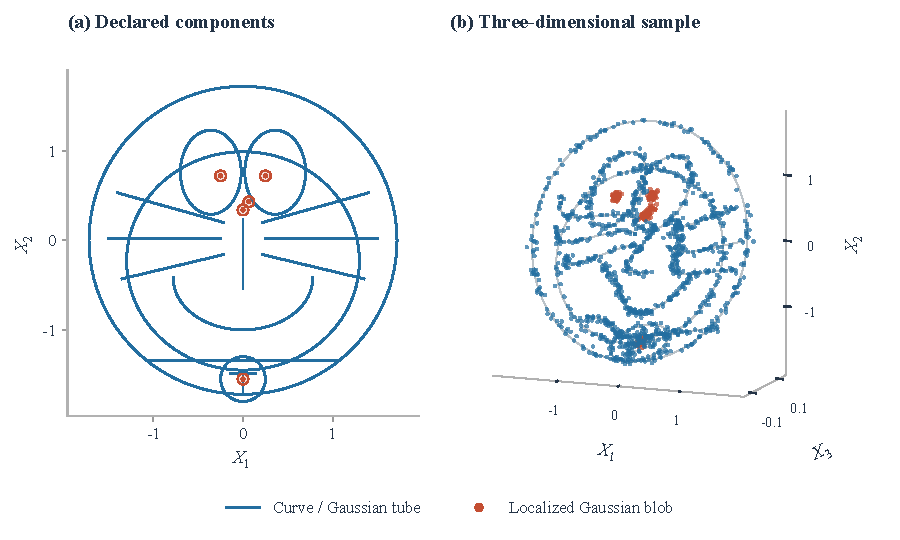
\includegraphics[width=0.93\linewidth,clip]{figures/face_example_3d.pdf}
\caption{A stylized-face SFD with 16 Gaussian tubes and five localized
Gaussian components. Left: projected centerlines and blob contours at
squared Mahalanobis distance four. Right: all 1,600 observations in three
dimensions, with gray centerlines as guides. Blue and red identify tubes
and blobs. Branch coordinates are uniform on $[0,1]$; SDs in the first two
coordinates are 0.020 for tubes and 0.030 for blobs, and the
third-coordinate SD is 0.012. The right panel uses actual $X_3$ values with
unequal display scales.}
\label{fig:face-example}
\end{figure}

\FloatBarrier


\section{Distributional Calculus}
\label{app:calculus}
All statements use the finite component sets and measurable kernels of
Definition~\ref{def:sfd}. Exact atoms are Dirac laws; regularized blobs can
be represented among the continuous residual components. Component labels
are latent and need not partition the observed space.

\begin{proposition}[Normalization and latent construction]
\label{prop:normalization}
The SFD law is the marginal of the following construction: draw a component
$Z$ with probabilities $\pi_c$; given an atom, set $X=\xi_a$; given a branch,
draw $S$ with density $h_b$ and then $X\sim K_b(\cdot\mid S)$; given a
residual, draw $X$ with density $q_r$. In particular, $P_\theta(\mathcal X)=1$.
\end{proposition}
\begin{proof}
Each branch integral is a measure: for disjoint measurable sets,
monotone convergence passes their sum through the nonnegative kernel
integral. It has total mass $\int h_b(s)K_b(\mathcal X\mid s)\,ds=1$.
The finite nonnegative mixture therefore has total mass $\sum_c\pi_c=1$.
Conditioning the stated latent construction on $Z$ gives exactly its
probability on every measurable set, proving equality of laws.
\end{proof}

\begin{proposition}[Mixed-density evaluation]
\label{prop:mixed-density}
For fixed atom locations and fixed exact branch maps, a common reference is
\[
 \nu=\lambda_d+\sum_a\delta_{\xi_a}
            +\sum_{b\in\mathcal B_{\mathrm{ex}}}(\gamma_b)_\#ds,
\]
where $ds$ is restricted to the finite-volume coordinate domain. If $P_c$
denotes each normalized component law, then
\[
 p_\theta=\sum_c\pi_c\frac{dP_c}{d\nu}.
\]
For a continuous component with Lebesgue density $g_c$, its common-reference
density is $g_c\rho$, where $\rho=d\lambda_d/d\nu$. For an injective exact
branch, put $\nu_{\Gamma,b}=(\gamma_b)_\#ds$. Its contribution is
\[
 \pi_b h_b\{\gamma_b^{-1}(x)\}
                    \frac{d\nu_{\Gamma,b}}{d\nu}(x).
\]
Thus overlapping reference contributions must be converted before addition.
\end{proposition}
\begin{proof}
The branch reference measures are finite and their finite sum with Lebesgue
measure is sigma-finite. A coordinate null set has zero probability under
$h_b(s)ds$, so its pushforward probability is dominated by its pushforward
reference. All components are therefore dominated by $\nu$. Linearity of
the Radon--Nikodym derivative gives the mixture formula; its chain rule gives
the continuous and injective-branch expressions. In particular, a continuous
density contributes zero mass at an exact atom, even if its Lebesgue density
there is positive.
\end{proof}

For a regular immersion of intrinsic dimension $m_b$ with finite preimages,
the area formula gives, at almost every point of its image,
\[
 \frac{dP_b}{d\mathcal H^{m_b}}(x)
   =\sum_{s:\gamma_b(s)=x}\frac{h_b(s)}{J_b(s)},\qquad
 J_b(s)=\sqrt{\det\{D\gamma_b(s)^\top D\gamma_b(s)\}}>0.
\]
Relative to the branch's own pushforward reference, the density is the ratio
of this sum to $\sum_{s:\gamma_b(s)=x}1/J_b(s)$, not the unweighted sum of
coordinate densities. The common-reference conversion still applies.

\subsection{Expectation, Moments and Covariance}
For completeness, Proposition~\ref{prop:expectation} follows first for
nonnegative $g$ by conditioning on $Z$, then $S$, and using Tonelli's theorem.
For integrable signed $g$, apply the same argument to $g^+$ and $g^-$ and
subtract. This proves the full identity without a Lebesgue-only assumption.

In the Gaussian-tube case, whenever the second moments exist,
\begin{align*}
 \mu=\E_\theta X
 &=\sum_a\pi_a\xi_a+\sum_b\pi_b\int h_b(s)\gamma_b(s)\,ds
                         +\sum_r\pi_r\E_{q_r}X,\\
 \E_\theta(XX^\top)
 &=\sum_a\pi_a\xi_a\xi_a^\top
   +\sum_b\pi_b\int h_b(s)
       \{\gamma_b(s)\gamma_b(s)^\top+\Sigma_b(s)\}\,ds
   +\sum_r\pi_r\E_{q_r}(XX^\top).
\end{align*}
The covariance is $\E_\theta(XX^\top)-\mu\mu^\top$. A branch covariance
therefore separates variation of $\gamma_b(S)$ from the average conditional
noise covariance $\int h_b(s)\Sigma_b(s)\,ds$. If the component moment
generating functions and the following integrals are finite near the origin,
\[
 M_X(t)=\sum_a\pi_a e^{t^\top\xi_a}
 +\sum_b\pi_b\int h_b(s)
   e^{t^\top\gamma_b(s)+t^\top\Sigma_b(s)t/2}\,ds
 +\sum_r\pi_r M_{q_r}(t).
\]
Both formulas are choices of $g$ in the master identity.

\subsection{Marginal and Conditional Laws}
Let $J$ be a nonempty proper subset of coordinate indices, put $Y=X_{-J}$,
and write $T_J$ for projection onto $X_J$.

\begin{proposition}[Marginal law]
\label{prop:marginal}
For arbitrary SFD kernels,
\[
 (T_J)_\#P_\theta
  =\sum_a\pi_a\delta_{\xi_{a,J}}
    +\sum_b\pi_b\int h_b(s)(T_J)_\#K_b(\cdot\mid s)\,ds
    +\sum_r\pi_r(T_J)_\#Q_r.
\]
For Gaussian tubes, the projected branch kernel is
$\Normal(\gamma_{b,J}(s),\Sigma_{b,JJ}(s))$. Exact branches instead use
their projected pushforward laws, which may change dimension or acquire atoms.
\end{proposition}
\begin{proof}
Evaluate the original law on $T_J^{-1}(A)$ for a measurable set $A$.
Projection commutes with the finite sum and nonnegative kernel integral.
The Gaussian assertion is the marginal formula for a multivariate normal.
\end{proof}

\begin{proposition}[Gaussian branch conditional law]
\label{prop:gaussian-conditional}
For a full-rank Gaussian branch kernel, conditional on $(Z=b,S=s,Y=y)$,
$X_J$ is Gaussian with mean and covariance
\begin{align*}
 m_{J\mid-J,b}(s;y)
 &=\gamma_{b,J}(s)+\Sigma_{b,J,-J}(s)\Sigma_{b,-J,-J}(s)^{-1}
                         \{y-\gamma_{b,-J}(s)\},\\
 V_{J\mid-J,b}(s)
 &=\Sigma_{b,JJ}(s)-\Sigma_{b,J,-J}(s)
            \Sigma_{b,-J,-J}(s)^{-1}\Sigma_{b,-J,J}(s).
\end{align*}
\end{proposition}
\begin{proof}
Positive definiteness makes the conditioning covariance block invertible.
Completing the square in the joint Gaussian density gives the displayed
mean and Schur-complement covariance.
\end{proof}

\begin{proposition}[Full conditional mixture]
\label{prop:full-conditional}
Choose a common projected reference $\nu_{-J}$ that dominates the projected
component laws and, for each regularized branch, its projected slice laws.
Let $g_{a,-J}$, $g_{b,-J}(y\mid s)$ and $g_{r,-J}$ be their densities
relative to this same reference, and let $p_{\theta,-J}$ be the total density.
For $P_{\theta,-J}$-almost every $y$ with positive density, put
\[
 \tau_a(y)=\frac{\pi_a g_{a,-J}(y)}{p_{\theta,-J}(y)},\qquad
 \tau_b(s\mid y)=\frac{\pi_bh_b(s)g_{b,-J}(y\mid s)}{p_{\theta,-J}(y)},
 \qquad
 \tau_r(y)=\frac{\pi_r g_{r,-J}(y)}{p_{\theta,-J}(y)}.
\]
For regularized branches and exact atoms, the full conditional law is
\begin{align*}
 \Pbb(X_J\in A\mid Y=y)
 &=\sum_a\tau_a(y)\mathbf 1_A(\xi_{a,J})\\
 &\quad+\sum_b\int \tau_b(s\mid y)
       K_{b,J\mid-J}(A\mid s,y)\,ds
       +\sum_r\tau_r(y)Q_{r,J\mid-J}(A\mid y).
\end{align*}
For Gaussian tubes the branch conditional is given by
Proposition~\ref{prop:gaussian-conditional}. Exact branches whose slice laws
lack common domination use a posterior coordinate measure obtained by
disintegration, rather than the displayed density relative to $ds$.
\end{proposition}
\begin{proof}
Disintegrate the joint latent-observed law with respect to $Y$. The three
Bayes numerators are its atom, branch-coordinate and residual contributions;
their sum/integral is $p_{\theta,-J}$. They therefore normalize to one.
Integrating each component's conditional law against these posterior weights
gives the assertion. The exceptional set is projected-law null, as required
for regular conditional distributions.
\end{proof}

For Gaussian slices under a mixed projected reference,
$g_{b,-J}(y\mid s)=\phi_{d-|J|}\{y;\gamma_{b,-J}(s),
\Sigma_{b,-J,-J}(s)\}\rho_{-J}(y)$, with
$\rho_{-J}=d\lambda_{d-|J|}/d\nu_{-J}$. That conversion also applies to
continuous residuals. Conditional simulation uses $\tau_b(s\mid y)$,
whereas full-observation EM uses $\tau_b(s\mid x)$; they condition on
different observations.

\subsection{Special-Case Embeddings}
\label{app:special-cases}
\begin{proposition}[Special-case status]
\label{prop:special-cases}
The following restrictions give exact equalities of laws or estimators.
\begin{enumerate}
\item Atoms alone give finite discrete distributions. An atom and a specified
continuous residual give the corresponding atom-inflated mixture.
\item Residual-only SFDs contain normal, product, heavy-tailed and finite
Gaussian-mixture laws by choosing the corresponding normalized $q_r$.
\item A residual-only mixture of $n$ fixed data-centered Gaussian kernels
with weights $1/n$ is exactly that KDE estimator.
\item One Gaussian tube gives Proposition~\ref{prop:single-tube}; specified
multiple tubes give mixtures of those laws. A Gaussian factor-analyzer
distribution enters as its integrated residual Gaussian density.
\item Exact kernels $\delta_{\gamma_b(s)}$ give coordinate-pushforward
laws under an intrinsic or mixed reference, not ambient Lebesgue densities.
\item A specified copula density with its marginal densities can be chosen
as a residual law. This does not identify SFD itself as a copula construction.
\end{enumerate}
A learned metric or temporal/path-functional model is an adjacent connection
until its extra structure is explicitly included in a normalized kernel or
dynamic extension.
\end{proposition}
\begin{proof}
Set inactive weights to zero and substitute the stated component laws in
Definition~\ref{def:sfd}. Each retained law is normalized. The KDE assertion
holds conditional on its chosen centers and bandwidth; it is an estimator
equality, not an additional parametric generating model. The pushforward
case is interpreted using Proposition~\ref{prop:mixed-density}. Extra
metric or temporal structure is not implied by a static mixture restriction.
\end{proof}

\section{Regular Likelihood Expansion and Contrast Tests}
\label{app:regular-theory}
This section proves Theorem~\ref{thm:regular-finite-sfd} for the whole
estimated finite chart, rather than holding estimated noise or geometry
fixed. The fixed component set and common support are part of its assumptions.

\subsection{Conditions for Theorem~\ref{thm:regular-finite-sfd}}
\label{app:regular-conditions}
Let $X_1,\ldots,X_n$ be iid from $P_{\theta_0}$ in a finite-dimensional
SFD family $p_\theta=dP_\theta/d\nu$. In an open neighborhood of the
interior parameter $\theta_0$, assume:
\begin{enumerate}
\item[\textup{(R1)}] The component set, atom supports, coordinate domains and effective
support are fixed, with one common dominating measure $\nu$.
\item[\textup{(R2)}] The chart is identifiable, active weights are bounded away from zero,
and active Gaussian tube covariance eigenvalues have positive lower and
finite upper bounds.
\item[\textup{(R3)}] The log density is $C^3$ almost everywhere on its support, its first
three derivatives have integrable local uniform envelopes, and derivatives
pass through branch integrals and integration against $\nu$.
\item[\textup{(R4)}] The score $U_0=\nabla\log p_{\theta_0}$ has finite, positive-definite
information $I_0=\E_{\theta_0}(U_0U_0^\top)$.
\item[\textup{(R5)}] An interior local likelihood maximizer $\hat\theta_n$ exists in this
chart with probability tending to one and is consistent for $\theta_0$.
\end{enumerate}
Consistency in (R5) is a separate input, not a consequence of local
smoothness. Data-selected topology, zero weights, moving singular supports
and covariance collapse require separate arguments. Transfer from a
numerical likelihood also needs score-error control at the root-$n$ scale
(Appendix~\ref{app:numerical-theory}).

\subsection{Proof of the Regular Finite-SFD Likelihood Theorem}
Write $P_nf=n^{-1}\sum_i f(X_i)$,
$U_0(x)=\nabla\log p_{\theta_0}(x)$ and
$H_0(x)=\nabla^2\log p_{\theta_0}(x)$. Differentiating normalization twice,
using the permitted integration interchanges, gives
\[
 \E_{\theta_0}U_0=0,\qquad
 \E_{\theta_0}H_0=-\E_{\theta_0}(U_0U_0^\top)=-I_0.
\]
The finite information assumption gives the score central limit theorem,
$\Delta_n=n^{-1/2}\sum_iU_0(X_i)\rightsquigarrow\Normal(0,I_0)$.
For any fixed $M<\infty$, Taylor's theorem and the third-derivative envelope
$M_3$ give, uniformly over $\|u\|\le M$,
\[
 \ell_n(\theta_0+u/\sqrt n)-\ell_n(\theta_0)
 =u^\top\Delta_n+\tfrac12u^\top(P_nH_0)u+R_n(u),
 \qquad \sup_{\|u\|\le M}|R_n(u)|
       \le C_Mn^{-1/2}P_nM_3=o_p(1).
\]
Since $P_nH_0\to_p-I_0$, this is the uniform local quadratic expansion
\begin{equation}
 \ell_n(\theta_0+u/\sqrt n)-\ell_n(\theta_0)
       =u^\top\Delta_n-\tfrac12u^\top I_0u+o_p(1).
 \label{eq:local-quadratic}
\end{equation}
Consistency and interiority give $\nabla\ell_n(\hat\theta_n)=0$ in a
neighborhood of $\theta_0$ with probability tending to one. Use the
segment-averaged Hessian, not a common scalar mean-value point:
\[
 \overline H_n=\frac1n\int_0^1
   \nabla^2\ell_n\{\theta_0+t(\hat\theta_n-\theta_0)\}\,dt.
\]
The fundamental theorem of calculus gives exactly
\[
 0=\Delta_n+\overline H_n\sqrt n(\hat\theta_n-\theta_0).
\]
The third-derivative envelope bounds
$\|\overline H_n-P_nH_0\|$ by a constant times
$\|\hat\theta_n-\theta_0\|P_nM_3=o_p(1)$, so
$\overline H_n\to_p-I_0$. Its inverse is bounded in probability.
Inverting the score equation first establishes root-$n$ consistency, then
the linear representation and Gaussian limit in
Equation~\ref{eq:regular-limit}. Differentiability of $\psi$ gives
\[
 \sqrt n\{\psi(\hat\theta_n)-\psi(\theta_0)\}
 =\dot\psi(\theta_0)I_0^{-1}\Delta_n+o_p(1),
\]
and hence the stated covariance. This proves the theorem.

\subsection{Smooth Contrasts}
For fixed component labels and coordinates, smooth targets include
$\pi_b$, $\sum_{a\in A_0}\pi_a$, $\int sh_b(s)\,ds$ and
$\int\operatorname{tr}\{\Sigma_{\perp,b}(s)\}h_b(s)\,ds$ when their
parameter derivatives exist. Independent group-specific fits can be combined
in one product chart; contrast variances then add the group contributions.
Coordinate-dependent targets also use the conventions of
Proposition~\ref{prop:coordinate-transport}.

\begin{proposition}[Regular tests for SFD contrasts]
\label{prop:regular-tests}
Under Theorem~\ref{thm:regular-finite-sfd}, let
$h:\Theta\to\R^q$ be $C^2$ near $\theta_0$ with full row-rank
$A=\dot h(\theta_0)$, and suppose $h(\theta_0)=0$. Let a constrained
local likelihood maximizer $\tilde\theta_n$ be consistent on this interior
null manifold, and let $\hat V_n\to_p I_0^{-1}$. Then
\begin{align*}
 W_n&=n h(\hat\theta_n)^\top
  \{\dot h(\hat\theta_n)\hat V_n\dot h(\hat\theta_n)^\top\}^{-1}
   h(\hat\theta_n)\ \rightsquigarrow\ \chi_q^2,\\
 \Lambda_n&=2\{\ell_n(\hat\theta_n)-\ell_n(\tilde\theta_n)\}
                  \ \rightsquigarrow\ \chi_q^2.
\end{align*}
\end{proposition}
\begin{proof}
Put $B=AI_0^{-1}A^\top\succ0$. The delta method gives
$\sqrt n h(\hat\theta_n)\rightsquigarrow\Normal(0,B)$, and the estimated
middle covariance tends to $B$. Its quadratic form proves the Wald result.

For the likelihood ratio, the $C^2$ full-rank null is locally a smooth
coordinate chart by the implicit function theorem. The same consistent
local-score argument as above, restricted to that chart, yields root-$n$
consistency of the constrained estimator. Its limiting tangent space is
$\mathcal T=\{u:Au=0\}$. Let $z_n=I_0^{-1}\Delta_n$ and define its
$I_0$-orthogonal projection
\[
 P_{\mathcal T}z=z-I_0^{-1}A^\top B^{-1}Az.
\]
Completing the square in Equation~\ref{eq:local-quadratic} shows that its
unrestricted and constrained maximizers are respectively $z_n$ and
$P_{\mathcal T}z_n$, up to $o_p(1)$. Root-$n$ consistency allows the
uniform compact expansion to be evaluated at both random maximizers.
Twice their quadratic maximum difference is therefore
\[
 \Lambda_n=(Az_n)^\top B^{-1}(Az_n)+o_p(1).
\]
Since $Az_n\rightsquigarrow\Normal(0,B)$, this tends to $\chi_q^2$.
\end{proof}

The $C^2$ null-chart assumption is stated explicitly for the likelihood-ratio
argument. A first-order differentiable contrast suffices for the Wald part.
These calibrations concern regular likelihood estimation in the specified
model; they do not calibrate zero weights, selected topology or singular
covariance limits.

\paragraph{Misspecification and penalties.}
For a consistent interior estimator targeting a regular population optimum
$\theta_*$ under a possibly misspecified law, an analogous centered-score
expansion gives covariance $H^{-1}JH^{-\top}$, where
$H=-\E\nabla^2\log p_{\theta_*}(X)$ and
$J=\E\{U_{\theta_*}(X)U_{\theta_*}(X)^\top\}$. This requires the
corresponding smoothness, nonsingularity and central-limit assumptions at
that target. A penalty with gradient $o_p(\sqrt n)$ and Hessian $o_p(n)$
locally leaves the first-order limit unchanged. A non-negligible penalty
instead changes the expansion or its centering. Neither a sandwich estimate
nor prior curvature repairs likelihood nonidentification.

\section{Finite-Grid Optimization and Approximation}
\label{app:numerical-theory}
\subsection{Proof of Fixed-Quadrature GEM Monotonicity}
For Proposition~\ref{prop:gem}, write $p_\theta(x,z)$ for the normalized
finite-grid joint density and $r_i(z)=p_{\theta^{\mathrm{old}}}(x_i,z)/
p_{\theta^{\mathrm{old}}}(x_i)$ for the old posterior. On labels with
$r_i(z)>0$, Jensen's inequality gives
\[
 \log p_\theta(x_i)\ge
  \sum_{z:r_i(z)>0}r_i(z)\log\frac{p_\theta(x_i,z)}{r_i(z)}.
\]
The bound is exact at the old iterate. Summing and subtracting the fixed
penalty gives $F_n(\theta)\ge Q(\theta\mid\theta^{\mathrm{old}})
-\operatorname{Pen}(\theta)+\sum_i\operatorname{Ent}(r_i)$.
The entropy is constant during the step. A nondecreasing penalized $Q$
therefore implies a nondecreasing observed objective. Zero old posterior
terms use $0\log0=0$; a proposed zero likelihood on a positive old posterior
cannot improve a finite auxiliary objective. The branch-node term uses
$\log\kappa_{bm}=\log w_{bm}+\log h_b(s_{bm})-\log C_b$ throughout.
Changing the grid or dropping its normalizer changes this argument's
objective and is not covered by the proposition.

\subsection{Numerical Likelihood and Root-n Inference}
\begin{proposition}[Transfer from a numerical likelihood]
\label{prop:numerical-transfer}
Under Theorem~\ref{thm:regular-finite-sfd}, let $\hat\theta_n$ be its
consistent interior exact-likelihood maximizer, and let $\tilde\theta_n$
be consistent for the same target under a differentiable numerical criterion
$\tilde\ell_n$. On a fixed neighborhood $N$ of $\theta_0$, assume
\[
 \|\nabla\tilde\ell_n(\tilde\theta_n)\|=o_p(\sqrt n),\qquad
 \sup_{\theta\in N}\|\nabla\tilde\ell_n(\theta)
                           -\nabla\ell_n(\theta)\|=o_p(\sqrt n).
\]
Then $\sqrt n(\tilde\theta_n-\hat\theta_n)=o_p(1)$. If also
\[
 \sup_{\theta\in N}n^{-1}\|\nabla^2\tilde\ell_n(\theta)
                           -\nabla^2\ell_n(\theta)\|=o_p(1),
\]
then $-n^{-1}\nabla^2\tilde\ell_n(\tilde\theta_n)\to_p I_0$.
\end{proposition}
\begin{proof}
The two score conditions give $\nabla\ell_n(\tilde\theta_n)=o_p(\sqrt n)$.
Subtract the zero exact score at $\hat\theta_n$ and integrate the exact
Hessian along their joining segment. Consistency and the local envelope
argument in Appendix~\ref{app:regular-theory} make that Hessian divided by
$n$ tend to $-I_0$. Inverting the score difference proves the estimator
claim. The additional Hessian discrepancy gives the information claim.
\end{proof}

The rates matter even for normalized densities. In the residual-only normal
submodel, take $p_\theta(x)=\phi_1(x;\theta,1)$ and
$\tilde p_{n,\theta}(x)=\phi_1(x;\theta+\epsilon_n,1)$ with
$\epsilon_n=n^{-1/4}$. Under iid $\Normal(0,1)$ data, the average criterion
difference vanishes uniformly on compact parameter sets, average scores
differ by $-\epsilon_n\to0$, and Hessians agree. Yet
$\tilde\theta_n-\hat\theta_n=-\epsilon_n$ and its root-$n$ multiple diverges.
Transfer to the continuous law requires average score error
$o_p(n^{-1/2})$, not just $o_p(1)$. A fixed normalized grid can instead be
treated as the statistical model in its own right.

\subsection{Mixture and Responsibility Perturbations}
\begin{proposition}[Mixture stability on a fixed stratum set]
\label{prop:mixture-stability}
Let $Q=\sum_c\pi_cQ_c$ and $\tilde Q=\sum_c\tilde\pi_c\tilde Q_c$ have
the same finite component index set. For
$d_{\mathrm{TV}}(P,Q)=\sup_A|P(A)-Q(A)|$,
\[
 d_{\mathrm{TV}}(Q,\tilde Q)\le
 \tfrac12\sum_c|\pi_c-\tilde\pi_c|
 +\sum_c(\pi_c\wedge\tilde\pi_c)d_{\mathrm{TV}}(Q_c,\tilde Q_c).
\]
If all components are supported on a set of diameter $D<\infty$, then for
$p\ge1$,
\[
 W_p^p(Q,\tilde Q)\le
 D^p\tfrac12\sum_c|\pi_c-\tilde\pi_c|
 +\sum_c(\pi_c\wedge\tilde\pi_c)W_p^p(Q_c,\tilde Q_c).
\]
\end{proposition}
\begin{proof}
Set $\alpha_c=\pi_c\wedge\tilde\pi_c$. Couple the shared mass $\alpha_c$
within component $c$ using a total-variation-optimal coupling. Couple the
remaining mass arbitrarily. Its total weight is
$1-\sum_c\alpha_c=\frac12\sum_c|\pi_c-\tilde\pi_c|$, giving the first
bound. For Wasserstein distance, use optimal or arbitrarily close-to-optimal
component couplings and transport the unmatched mass at cost at most $D^p$
per unit mass. Taking the infimum gives the second bound. The diameter
assumption is not asserted for unbounded Gaussian tubes.
\end{proof}

\begin{proposition}[Relative quadrature error controls log likelihood]
\label{prop:relative-quadrature}
Suppose $p_\theta(x_i)$ and $\tilde p_\theta(x_i)$ are finite and positive
and, uniformly over $\theta\in\Theta_0$ and all observations,
\[
 \left|\tilde p_\theta(x_i)/p_\theta(x_i)-1\right|\le\epsilon<1.
\]
Then
\[
 \sup_{\theta\in\Theta_0}|\tilde\ell_n(\theta)-\ell_n(\theta)|
       \le-n\log(1-\epsilon)\le2n\epsilon
       \quad\text{if }\epsilon\le1/2.
\]
\end{proposition}
\begin{proof}
Each density ratio lies between $1-\epsilon$ and $1+\epsilon$. Take
logarithms, sum, and use $\log(1+\epsilon)\le-\log(1-\epsilon)$.
The last bound follows from $-\log(1-\epsilon)\le2\epsilon$ on $[0,1/2]$.
This is a criterion bound; it does not establish the score rates in
Proposition~\ref{prop:numerical-transfer}.
\end{proof}

\begin{proposition}[Softmax responsibility perturbation]
\label{prop:softmax-perturbation}
For finite log-score vectors $a,\tilde a$, let
$r_z=e^{a_z}/\sum_u e^{a_u}$ and
$\tilde r_z=e^{\tilde a_z}/\sum_u e^{\tilde a_u}$.
If $\max_z|a_z-\tilde a_z|\le\delta$, then
\[
 e^{-2\delta}\le\tilde r_z/r_z\le e^{2\delta},\qquad
 \sum_z|\tilde r_z-r_z|\le e^{2\delta}-1.
\]
\end{proposition}
\begin{proof}
Exponentiation bounds each numerator ratio by $e^{\pm\delta}$; summation
gives the same bounds for the normalizing-constant ratio. Division gives
$e^{\pm2\delta}$. Thus
$|\tilde r_z-r_z|\le(e^{2\delta}-1)r_z$; summing proves the result.
\end{proof}

\section{Tube-Distance Concentration}
\label{app:tube-tails}
This result isolates the probability of leaving a declared tube from the
geometric distance estimate used to define that tube. In particular, a
positive reach condition alone is not a derivation of a residual bound.

\begin{proposition}[Tube-distance concentration from residual tails]
\label{prop:tube-concentration}
Let $\Gamma_b=\gamma_b(\mathcal S_b)$ and
$d_{\Gamma_b}(x)=\inf_{y\in\Gamma_b}\|x-y\|$. On a measurable coordinate
subset $U_b$ of positive branch-coordinate probability, suppose the observation is
$X=\gamma_b(S)+t_b(S)\varepsilon_{\parallel,b}
+N_b(S)\varepsilon_{\perp,b}$. Let
$0<M_{N,b}=\sup_{s\in U_b}\|N_b(s)\|_{\mathrm{op}}<\infty$.
Assume a nonnegative measurable remainder $R_b$ and radius $\rho_b>0$
satisfy
\[
 d_{\Gamma_b}(X)\le M_{N,b}\|\varepsilon_{\perp,b}\|+R_b
 \quad\text{whenever }S\in U_b\text{ and }
 M_{N,b}\|\varepsilon_{\perp,b}\|+R_b<\rho_b.
\]
For $0<r<\rho_b$ and $0<\eta<1$, set $a=(1-\eta)r/M_{N,b}$ and
\begin{align*}
 \Delta_b(r,\eta)
 &=\Pbb(S\notin U_b\mid Z=b)\\
 &\quad+\operatorname*{ess\,sup}_{s\in U_b}
          \Pbb(\|\varepsilon_{\perp,b}\|>a\mid S=s,Z=b)\\
 &\quad+\operatorname*{ess\,sup}_{s\in U_b}
          \Pbb(R_b>\eta r\mid S=s,Z=b).
\end{align*}
Essential suprema use the branch-coordinate law. Then
\[
 \Pbb\{d_{\Gamma_b}(X)>r\mid Z=b\}\le\Delta_b(r,\eta).
\]
For $n_b$ observations conditional on branch $b$, the probability that at
least one leaves the radius-$r$ tube is at most $n_b\Delta_b(r,\eta)$.
For $n$ draws from the mixture and an active branch subset $\mathcal B_0$,
\[
 \Pbb\{\exists i:Z_i\in\mathcal B_0,
                  d_{\Gamma_{Z_i}}(X_i)>r\}
       \le n\sum_{b\in\mathcal B_0}\pi_b\Delta_b(r,\eta).
\]
\end{proposition}
\begin{proof}
If $S\in U_b$, $\|\varepsilon_{\perp,b}\|\le a$ and $R_b\le\eta r$,
the assumed bound is at most $r<\rho_b$. The escape event is therefore
contained in the union of the three complement events in $\Delta_b$.
Conditioning on $S$ and applying the union bound proves the first assertion.
Union bounds over observations and then mixture labels give the other two.
They do not require independence beyond the stated one-observation laws.
\end{proof}

\begin{corollary}[Gaussian residual-tail specialization]
\label{cor:gaussian-tube-tail}
In Proposition~\ref{prop:tube-concentration}, suppose conditionally on $S=s$
that $\varepsilon_{\perp,b}=A_b(s)G$ with
$G\sim\Normal(0,I_{r_b^{\varepsilon}})$. Set
\[
 \bar m_b=\operatorname*{ess\,sup}_{s\in U_b}\E\|A_b(s)G\|,
 \qquad
 \bar\sigma_b=\operatorname*{ess\,sup}_{s\in U_b}\|A_b(s)\|_{\mathrm{op}}.
\]
If $0<\bar\sigma_b<\infty$, the normal-residual term in $\Delta_b$ is
bounded by
\[
 \exp\left\{-\frac{(a-\bar m_b)_+^2}{2\bar\sigma_b^2}\right\}.
\]
If $\bar\sigma_b=0$, that term is zero for $a>0$.
\end{corollary}
\begin{proof}
For fixed $s$, the Gaussian function $g\mapsto\|A_b(s)g\|$ is
$\|A_b(s)\|_{\mathrm{op}}$-Lipschitz. Gaussian Lipschitz concentration
\citep{boucheron2013concentration} bounds its upper tail above its mean
by $\exp\{-t^2/(2\|A_b(s)\|_{\mathrm{op}}^2)\}$ for $t\ge0$.
Use the trivial bound one when $a$ is below the mean, otherwise take
$t=a-\E\|A_b(s)G\|$. Uniform bounds on the mean and Lipschitz constant
give the display. Zero operator norm gives zero residual almost surely.
\end{proof}

Other observation kernels enter the same first proposition through their
own residual tails. It is the kernel law and the assumed geometric remainder,
not the name of the mixture family, that determine concentration.


\section{Experiment Details}
\label{app:experiments}
The following settings define the four studies in Section~\ref{sec:experiments}.
Numerical summaries use all recorded repetitions and retain the convergence
status of every selected fit. The supplementary tables report the full
prespecified density and marker controls.

\paragraph{Known-skeleton weight diagnostic.}
The five generating laws and component families are fixed before fitting.
Each of 25 repetitions uses 1000 training and 1000 independent test
observations. EM estimates component weights with a 64-node tube grid,
a maximum of 300 iterations, maximum-weight-change tolerance $10^{-6}$
and minimum weight $10^{-12}$. Gaussian, KDE and GMM controls share the
observations; GMM sizes are $2,4,8,16,32$, with maximum 80 iterations,
tolerance $10^{-5}$ and covariance regularization $10^{-5}$.
The base seed is 20260623, with repetition offset $10000$ and
zero-based scenario offset $101$. The archived per-run and summary tables
retain every method, convergence status and recovery result. This experiment
does not estimate the skeleton, tube width or latent-coordinate error.

\paragraph{Two-arm study.}
The location $\mu_b^{\mathrm{loc}}$ is a truncated-normal parameter, not the
coordinate mean. The mean-position contrast changes it from $0.5$ to $0.7$
at scale $0.16$ on $[0,1]$, giving a generating mean contrast of about $0.189$.
Longitudinal convolution with tangent Gaussian noise has a closed form.
The direct optimizer is L-BFGS-B with maxiter 300, ftol $10^{-10}$, gtol
$10^{-6}$, maxls 40, mass-logit bounds $[-5,5]$, location bounds $[0.1,0.9]$,
and width bounds $[0.025,0.3]$. Every method and repetition is retained below;
the oracle row is a generating-density reference, not a fitted competitor.
The archived score rows also retain the observable $\Pbb(X_2>0)$ comparison
and all convergence flags, including GMM iteration limits.

\paragraph{Geometry and noise study.}
The learned directions are bounded to $[5,75]$ and $[-75,-5]$ degrees. Three
starts use angle pairs $\pm20$, $\pm35$, $\pm50$ degrees, with the recorded
location and width starts. L-BFGS-B uses maxiter 500 and the same tolerances.
The best finite training objective selects the fit. GMM uses three separately
seeded starts, covariance regularization $10^{-5}$, maxiter 2000 and tol
$10^{-5}$. KDE chooses $0.5$, $1$, or $2$ times Scott's bandwidth on a
deterministic 80/20 inner split, then refits on all training rows. The outer
test set is never used for selection.

\paragraph{PBMC prediction diagnostic.}
The analysis uses the public 10x PBMC3k filtered count matrix. Filtering keeps
genes detected in at least three
training cells, and selects the 1000 largest training log-CP10k variances,
breaking ties by gene index. Training means and SDs scale the data, values
are clipped to $[-10,10]$, and randomized PCA has two components. All
18 predeclared marker genes are excluded from predictor normalization and
selection. Marker-group means use the same nonmarker library size. A cell is
positive when the B-marker mean log-CP10k is at least $0.5$ and strictly
exceeds each competing marker-group mean. This fixed rule precedes the
repeated analysis.

The MST model uses 24 landmarks and 12 quadrature nodes with the archived
width/residual heuristic. Its small-mass-change stopping rule is not a joint
objective certificate. All density controls and readouts share the outer
train/test representation. Logistic predictors select inverse L2 penalty
from $\{0.01,0.1,1,10\}$ on the same stratified 75/25 inner training split,
then refit all outer training cells. Dropping the eighth GMM posterior
coordinate removes exact simplex redundancy. The two-coordinate density and
marker readouts concern cell-level prediction within one collection;
independent-donor and externally annotated validation are separate tasks.

\section{Parameter Intervals for the Saved Fits}
\label{app:intervals}
The post-hoc interval diagnostic reuses all \GeoFitCount{} saved SFD fits
from the geometry/noise study: 600 use six parameters and 300 include the
two estimated angles. The chart contains two mass logits relative to the
residual, two coordinate-normal locations, two log transverse SDs, and the
two angles when active. The origin, coordinate/tangent scales, residual law,
and two-arm family remain supplied. No fit is repeated, and no test
observations enter the interval calculation.

Let $H=\left.\nabla_\theta^2\{-\ell_n(\theta)/n\}\right|_{\theta=\hat\theta}$
and $U_i=\left.\nabla_\theta\log p_\theta(X_i)\right|_{\theta=\hat\theta}$.
With $J=n^{-1}\sum_i U_iU_i^\top$, the two covariance estimates are
\[
 \widehat V_{\mathrm{info}}=H^{-1}/n,\qquad
 \widehat V_{\mathrm{sand}}=H^{-1}JH^{-\top}/n.
\]
The inverse uses the complete fitted chart; estimated angles are not held
fixed. For a target $\psi$, the delta-method variance is
$\dot\psi(\hat\theta)\widehat V\dot\psi(\hat\theta)^\top$.
The mass gradient uses the softmax row. The truncated-coordinate-mean
derivative with respect to its normal location is
$\operatorname{Var}(S\mid Z=+)/0.16^2$; the SD derivative with respect to
log SD is $\sigma_+$. Contrasts add the independent alternative and reference
variances. Intervals are untransformed normal Wald intervals without clipping.
The three contrasts within a repetition share the reference fit.

\paragraph{Numerical checks.}
The original 300 training arrays regenerate identically. Source-version,
saved-objective and target checks precede inference. Central differences of
the average-loss gradient use relative steps $10^{-4}$, $5\times10^{-5}$,
and $2.5\times10^{-5}$. Relative Hessian changes and asymmetry must be at
most $5\times10^{-5}$; the information eigenvalues must exceed $10^{-8}$
and the condition number must be below $10^8$ in the stated chart. Fit and
perturbed parameters remain interior, and maximum average-score magnitude
must be at most $10^{-4}$. No ridge or pseudoinverse repairs a failed matrix.
All 900 saved fits pass these gates.

An independent audit constructs scalar-likelihood Hessians using relative
steps $4\times10^{-4}$ and $2\times10^{-4}$ with Richardson cancellation.
It uses numerical individual log-density derivatives and target derivatives
at step $10^{-5}$, rather than the analytic scores or production target
Jacobian. All group-target standard errors agree with the saved-fit
calculation under mixed relative/absolute tolerance $5\times10^{-5}$ and
$10^{-9}$. Coverage, contrast variances and every summary cell are
independently recounted. The complete record retains
\GeoIntervalCount{} group/contrast intervals and \GeoSummaryCount{} summary
cells, each with 25 repetitions and zero invalid fits. Intervals from the
same fit or shared reference are not pooled as independent trials.

\paragraph{Interpretation.}
Coverage refers to the generating targets, including under rotated geometry
or Student-$t_5$ noise. A sandwich covariance estimates variation around a
pseudo-true target under the corresponding regularity assumptions; it does
not remove its discrepancy from the generating parameter. Figure~\ref{fig:intervals}
and Table~\ref{tab:geometry-intervals} show every intended contrast/target
pair. The accompanying summary data also retain all group parameters and
cross-effects. With 25 repetitions, coverage is imprecisely estimated;
even a count of 25/25 does not establish nominal calibration. This diagnostic
accounts for two estimated directions, not topology selection or a general
learned skeleton.

\begin{figure}[tbp]
\centering
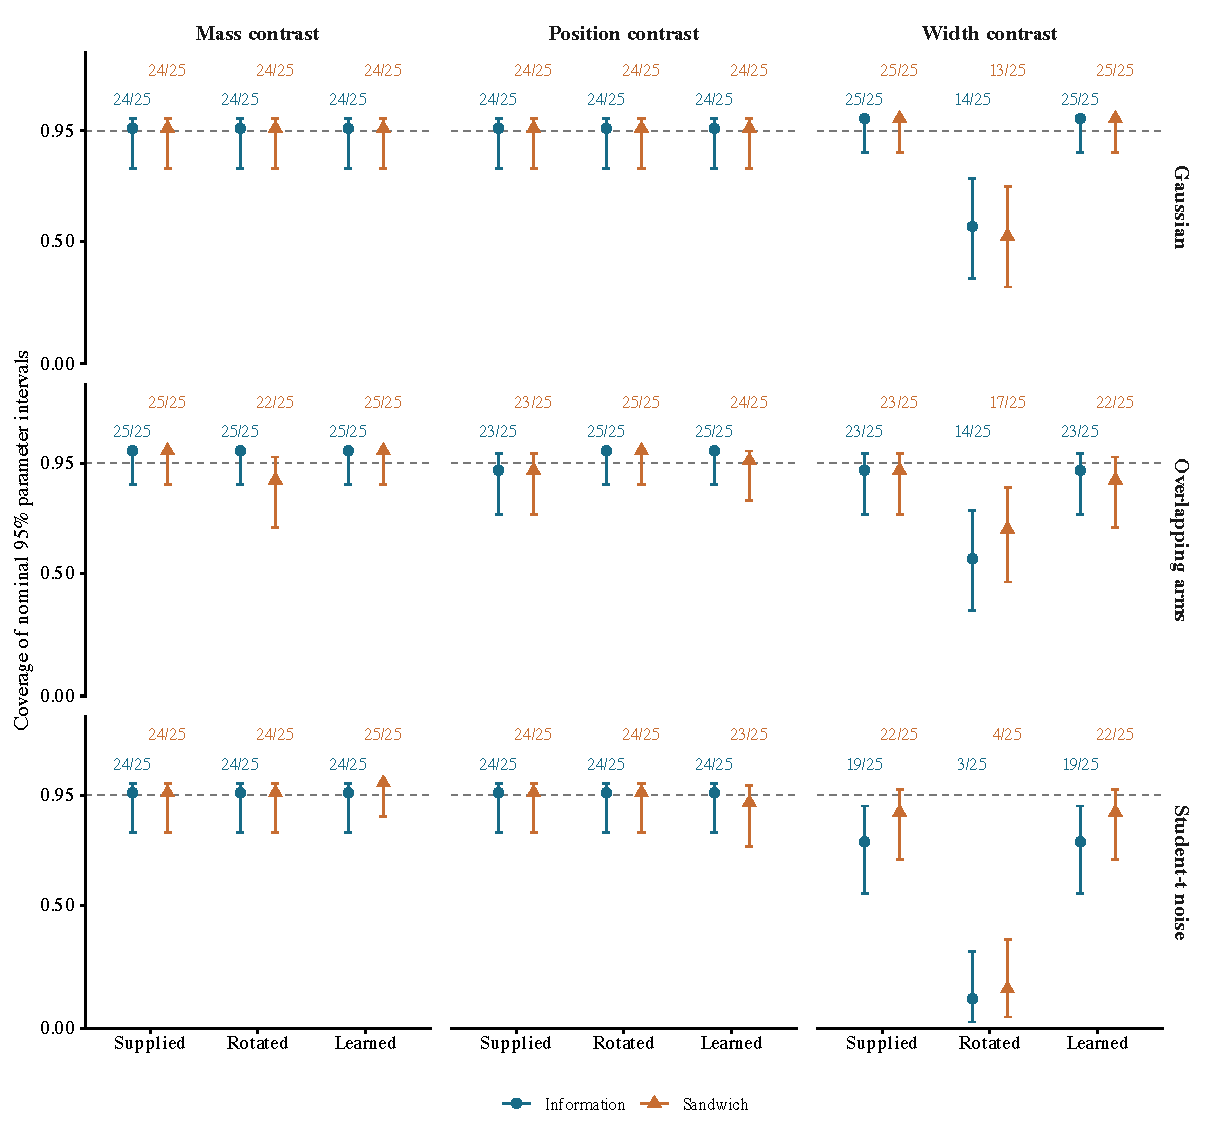
\includegraphics[width=\textwidth,clip]{figures/geometry_interval_coverage.pdf}
\caption{Post-hoc coverage of nominal 95\% parameter intervals for the
geometry/noise study. Columns show the three intended mass, coordinate-mean
and transverse-SD contrasts; rows show Gaussian noise, overlapping arms,
and equal-SD Student-$t_5$ noise. Points and counts use all 25 repetitions.
Bars are exact binomial 95\% Monte Carlo intervals for coverage, not parameter
intervals; the dashed line marks 0.95. Both covariance choices use the same
saved fit and complete six/eight-parameter chart. The 54 displayed cells
follow the prespecified contrast/target pairs; the full numerical record
retains all 378 cells.}
\label{fig:intervals}
\end{figure}

\begin{table}[tbp]
\centering
\footnotesize
\setlength{\tabcolsep}{3pt}
\caption{All intended contrast/target pairs in the saved geometry fits.
Info. and Sand. give covered intervals out of 25 for information and sandwich
covariance. Bias is the mean estimate minus the generating contrast; it is
the same for both covariance choices. SE columns are mean parameter standard
errors, not Monte Carlo SEs. Position is the truncated coordinate mean; SD
is transverse spread. Cross-effects remain in the accompanying complete data.}
\label{tab:geometry-intervals}
\begin{tabular}{@{}lllrrrrr@{}}
\toprule
Condition & Directions & Target & Info. & Sand. & Bias & SE (info.) & SE (sand.) \\
\midrule
Gaussian & Supplied & Mass & 24/25 & 24/25 & 0.00752 & 0.02354 & 0.02354 \\
Gaussian & Supplied & Position & 24/25 & 24/25 & 0.00173 & 0.01186 & 0.01173 \\
Gaussian & Supplied & SD & 25/25 & 25/25 & 0.00153 & 0.00733 & 0.00730 \\
\addlinespace[3pt]
Gaussian & Rotated & Mass & 24/25 & 24/25 & 0.00830 & 0.02389 & 0.02387 \\
Gaussian & Rotated & Position & 24/25 & 24/25 & -0.00048 & 0.01206 & 0.01178 \\
Gaussian & Rotated & SD & 14/25 & 13/25 & -0.01342 & 0.00751 & 0.00716 \\
\addlinespace[3pt]
Gaussian & Learned & Mass & 24/25 & 24/25 & 0.00756 & 0.02354 & 0.02355 \\
Gaussian & Learned & Position & 24/25 & 24/25 & 0.00171 & 0.01186 & 0.01174 \\
Gaussian & Learned & SD & 25/25 & 25/25 & 0.00154 & 0.00738 & 0.00738 \\
\addlinespace[3pt]
Overlap & Supplied & Mass & 25/25 & 25/25 & 0.00697 & 0.02596 & 0.02601 \\
Overlap & Supplied & Position & 23/25 & 23/25 & -0.00149 & 0.01268 & 0.01268 \\
Overlap & Supplied & SD & 23/25 & 23/25 & 0.00305 & 0.00906 & 0.00903 \\
\addlinespace[3pt]
Overlap & Rotated & Mass & 25/25 & 22/25 & 0.01863 & 0.02954 & 0.02859 \\
Overlap & Rotated & Position & 25/25 & 25/25 & 0.00185 & 0.01549 & 0.01505 \\
Overlap & Rotated & SD & 14/25 & 17/25 & -0.01498 & 0.01001 & 0.01069 \\
\addlinespace[3pt]
Overlap & Learned & Mass & 25/25 & 25/25 & 0.00497 & 0.02733 & 0.02744 \\
Overlap & Learned & Position & 25/25 & 24/25 & -0.00135 & 0.01280 & 0.01281 \\
Overlap & Learned & SD & 23/25 & 22/25 & 0.00385 & 0.01191 & 0.01211 \\
\addlinespace[3pt]
Student-$t_5$ & Supplied & Mass & 24/25 & 24/25 & -0.00972 & 0.02373 & 0.02386 \\
Student-$t_5$ & Supplied & Position & 24/25 & 24/25 & 0.00281 & 0.01191 & 0.01183 \\
Student-$t_5$ & Supplied & SD & 19/25 & 22/25 & -0.00655 & 0.00713 & 0.00819 \\
\addlinespace[3pt]
Student-$t_5$ & Rotated & Mass & 24/25 & 24/25 & -0.00688 & 0.02396 & 0.02396 \\
Student-$t_5$ & Rotated & Position & 24/25 & 24/25 & 0.00064 & 0.01203 & 0.01186 \\
Student-$t_5$ & Rotated & SD & 3/25 & 4/25 & -0.02203 & 0.00722 & 0.00760 \\
\addlinespace[3pt]
Student-$t_5$ & Learned & Mass & 24/25 & 25/25 & -0.00979 & 0.02374 & 0.02387 \\
Student-$t_5$ & Learned & Position & 24/25 & 23/25 & 0.00283 & 0.01191 & 0.01183 \\
Student-$t_5$ & Learned & SD & 19/25 & 22/25 & -0.00645 & 0.00718 & 0.00830 \\
\addlinespace[3pt]
\bottomrule
\end{tabular}

\end{table}

\paragraph{Fixed directions in the original mechanism study.}
A separate post-hoc calculation uses all 100 joint fits from the earlier
mechanism study. Its complete six-parameter covariance gives 300 group-target
and 225 contrast-target intervals with no invalid fits. Table~\ref{tab:fixed-intervals}
retains all 21 summary cells. These are different saved fits from those in
the geometry/noise study; their repetitions are not pooled.

\begin{table}[tbp]
\centering
\footnotesize
\setlength{\tabcolsep}{3pt}
\caption{Complete fixed-direction joint-fit interval diagnostic. Covered
counts use 25 repetitions per row. MC intervals are exact binomial 95\%
intervals for coverage; empirical SD and mean SE concern the parameter or
contrast estimator. Contrast rows subtract the independently sampled
reference group. None of these rows describes learned-direction uncertainty.}
\label{tab:fixed-intervals}
\begin{tabular}{@{}lllrrrr@{}}
\toprule
Scope & Group & Target & Covered & 95\% MC interval & Empirical SD & Mean SE \\
\midrule
Group & Reference & Mass & 24/25 & [0.796, 0.999] & 0.01738 & 0.01670 \\
Group & Reference & Position & 24/25 & [0.796, 0.999] & 0.00823 & 0.00870 \\
Group & Reference & Width & 22/25 & [0.688, 0.975] & 0.00369 & 0.00309 \\
\addlinespace[3pt]
Group & Mass & Mass & 22/25 & [0.688, 0.975] & 0.02092 & 0.01673 \\
Group & Mass & Position & 25/25 & [0.863, 1.000] & 0.00486 & 0.00697 \\
Group & Mass & Width & 24/25 & [0.796, 0.999] & 0.00189 & 0.00240 \\
\addlinespace[3pt]
Group & Position & Mass & 24/25 & [0.796, 0.999] & 0.01324 & 0.01637 \\
Group & Position & Position & 24/25 & [0.796, 0.999] & 0.00794 & 0.00810 \\
Group & Position & Width & 25/25 & [0.863, 1.000] & 0.00285 & 0.00298 \\
\addlinespace[3pt]
Group & Width & Mass & 24/25 & [0.796, 0.999] & 0.01758 & 0.01798 \\
Group & Width & Position & 25/25 & [0.863, 1.000] & 0.00972 & 0.00932 \\
Group & Width & Width & 24/25 & [0.796, 0.999] & 0.00713 & 0.00669 \\
\addlinespace[3pt]
Contrast & Mass & Mass & 22/25 & [0.688, 0.975] & 0.02711 & 0.02364 \\
Contrast & Mass & Position & 25/25 & [0.863, 1.000] & 0.00884 & 0.01115 \\
Contrast & Mass & Width & 24/25 & [0.796, 0.999] & 0.00380 & 0.00392 \\
\addlinespace[3pt]
Contrast & Position & Mass & 24/25 & [0.796, 0.999] & 0.02030 & 0.02338 \\
Contrast & Position & Position & 23/25 & [0.740, 0.990] & 0.01095 & 0.01189 \\
Contrast & Position & Width & 23/25 & [0.740, 0.990] & 0.00515 & 0.00430 \\
\addlinespace[3pt]
Contrast & Width & Mass & 24/25 & [0.796, 0.999] & 0.02332 & 0.02454 \\
Contrast & Width & Position & 23/25 & [0.740, 0.990] & 0.01417 & 0.01275 \\
Contrast & Width & Width & 24/25 & [0.796, 0.999] & 0.00826 & 0.00737 \\
\bottomrule
\end{tabular}

\end{table}
\FloatBarrier

\section{All Prespecified Density and Marker Controls}
\label{app:controls}
Every cell below is mean (Monte Carlo SE) over 25 runs. Density scores are
in nats per observation; higher is better. Marker log loss is lower-is-better.
PBMC differences are paired within split, and their SEs describe split
variability in this one collection. No independent-subject uncertainty is
estimated. Simulation score tables retain the same observations per method;
the supplied structural information differs between the SFD ablations and
generic density controls as described in the main text.

\begingroup
\let\paragraph\subsubsection
\subsection{Fixed-geometry density scores}

\begin{tabular}{lrrrr}\toprule
Method & Reference & Mass & Position & Width \\\midrule
Oracle & \numSE{0.146}{0.007} & \numSE{0.232}{0.008} & \numSE{0.144}{0.007} & \numSE{-0.079}{0.008} \\
SFD joint & \numSE{0.143}{0.007} & \numSE{0.229}{0.008} & \numSE{0.142}{0.007} & \numSE{-0.083}{0.008} \\
SFD fixed kernels & \numSE{0.145}{0.007} & \numSE{0.231}{0.008} & \numSE{-0.095}{0.008} & \numSE{-0.179}{0.007} \\
SFD oracle kernels & \numSE{0.145}{0.007} & \numSE{0.231}{0.008} & \numSE{0.143}{0.007} & \numSE{-0.080}{0.008} \\
Gaussian & \numSE{-0.475}{0.007} & \numSE{-0.451}{0.008} & \numSE{-0.601}{0.009} & \numSE{-0.528}{0.009} \\
GMM-4 & \numSE{0.132}{0.007} & \numSE{0.218}{0.008} & \numSE{0.129}{0.007} & \numSE{-0.095}{0.008} \\
GMM-8 & \numSE{0.111}{0.007} & \numSE{0.194}{0.008} & \numSE{0.109}{0.008} & \numSE{-0.117}{0.009} \\
KDE & \numSE{-0.078}{0.009} & \numSE{0.007}{0.008} & \numSE{-0.114}{0.009} & \numSE{-0.240}{0.010} \\
\bottomrule\end{tabular}

\subsection{Geometry/noise density scores}

\paragraph{Gaussian noise.}

\begin{tabular}{lrrrr}\toprule
Method & Reference & Mass & Position & Width \\\midrule
SFD supplied & \numSE{0.123}{0.006} & \numSE{0.226}{0.007} & \numSE{0.142}{0.010} & \numSE{-0.088}{0.007} \\
SFD rotated & \numSE{0.010}{0.005} & \numSE{0.109}{0.008} & \numSE{-0.020}{0.008} & \numSE{-0.152}{0.007} \\
SFD learned angles & \numSE{0.122}{0.006} & \numSE{0.225}{0.007} & \numSE{0.141}{0.010} & \numSE{-0.089}{0.007} \\
Gaussian & \numSE{-0.496}{0.005} & \numSE{-0.454}{0.011} & \numSE{-0.602}{0.008} & \numSE{-0.537}{0.009} \\
GMM-4 & \numSE{0.112}{0.006} & \numSE{0.216}{0.008} & \numSE{0.128}{0.010} & \numSE{-0.101}{0.007} \\
GMM-8 & \numSE{0.088}{0.007} & \numSE{0.193}{0.008} & \numSE{0.105}{0.012} & \numSE{-0.127}{0.008} \\
KDE & \numSE{-0.111}{0.016} & \numSE{-0.001}{0.019} & \numSE{-0.165}{0.020} & \numSE{-0.263}{0.011} \\
\bottomrule\end{tabular}

\paragraph{Overlapping arms.}

\begin{tabular}{lrrrr}\toprule
Method & Reference & Mass & Position & Width \\\midrule
SFD supplied & \numSE{0.199}{0.008} & \numSE{0.289}{0.011} & \numSE{0.166}{0.005} & \numSE{0.067}{0.005} \\
SFD rotated & \numSE{0.139}{0.008} & \numSE{0.212}{0.010} & \numSE{0.045}{0.006} & \numSE{0.043}{0.005} \\
SFD learned angles & \numSE{0.198}{0.008} & \numSE{0.288}{0.011} & \numSE{0.165}{0.005} & \numSE{0.065}{0.005} \\
Gaussian & \numSE{-0.326}{0.011} & \numSE{-0.307}{0.013} & \numSE{-0.401}{0.011} & \numSE{-0.360}{0.008} \\
GMM-4 & \numSE{0.185}{0.009} & \numSE{0.277}{0.011} & \numSE{0.153}{0.006} & \numSE{0.055}{0.005} \\
GMM-8 & \numSE{0.165}{0.008} & \numSE{0.253}{0.011} & \numSE{0.132}{0.006} & \numSE{0.030}{0.006} \\
KDE & \numSE{0.009}{0.013} & \numSE{0.085}{0.017} & \numSE{-0.023}{0.011} & \numSE{-0.074}{0.008} \\
\bottomrule\end{tabular}

\paragraph{Student-t noise.}

\begin{tabular}{lrrrr}\toprule
Method & Reference & Mass & Position & Width \\\midrule
SFD supplied & \numSE{0.157}{0.007} & \numSE{0.264}{0.008} & \numSE{0.173}{0.008} & \numSE{-0.043}{0.007} \\
SFD rotated & \numSE{0.023}{0.006} & \numSE{0.130}{0.008} & \numSE{-0.005}{0.007} & \numSE{-0.121}{0.007} \\
SFD learned angles & \numSE{0.157}{0.007} & \numSE{0.263}{0.008} & \numSE{0.173}{0.008} & \numSE{-0.044}{0.007} \\
Gaussian & \numSE{-0.510}{0.008} & \numSE{-0.450}{0.009} & \numSE{-0.611}{0.007} & \numSE{-0.522}{0.007} \\
GMM-4 & \numSE{0.148}{0.007} & \numSE{0.257}{0.009} & \numSE{0.160}{0.008} & \numSE{-0.052}{0.007} \\
GMM-8 & \numSE{0.129}{0.007} & \numSE{0.236}{0.009} & \numSE{0.138}{0.008} & \numSE{-0.075}{0.007} \\
KDE & \numSE{-0.184}{0.040} & \numSE{-0.035}{0.037} & \numSE{-0.171}{0.026} & \numSE{-0.224}{0.007} \\
\bottomrule\end{tabular}

\subsection{PBMC density and marker controls}

\begin{tabular}{lr}\toprule Method & Test log density \\\midrule

Gaussian & \numSE{-6.422}{0.006} \\

GMM-2 & \numSE{-5.649}{0.011} \\

GMM-4 & \numSE{-5.415}{0.010} \\

GMM-8 & \numSE{-5.367}{0.009} \\

KDE & \numSE{-5.421}{0.009} \\

MST SFD & \numSE{-5.770}{0.018} \\

\bottomrule\end{tabular}

\begin{tabular}{lrr}\toprule Readout & Log loss & Change vs density \\\midrule

PCs & \numSE{0.2526}{0.0036} & \numSE{0.0017}{0.0006} \\

PCs + density & \numSE{0.2509}{0.0033} & \numSE{0.0000}{0.0000} \\

PCs + density + entropy & \numSE{0.2257}{0.0041} & \numSE{-0.0252}{0.0032} \\

PCs + density + SFD & \numSE{0.2029}{0.0056} & \numSE{-0.0481}{0.0044} \\

PCs + density + GMM memberships & \numSE{0.1544}{0.0024} & \numSE{-0.0965}{0.0030} \\

\bottomrule\end{tabular}

\endgroup

\FloatBarrier
\clearpage
\section{External-Family Density Controls}
\label{app:external-density-controls}
These two archived comparisons characterize generic density estimators on
classical and copula distributions. Each uses five repetitions with 1000
training and 1000 independent test observations per scenario. Oracle rows
evaluate the known generating density; neither comparison fits an SFD.
The full score and summary tables accompany the compilation sources.
Finite scores from runs with iteration-limit warnings remain in the means;
the archived status columns identify those runs.

\begin{figure}[H]
\centering
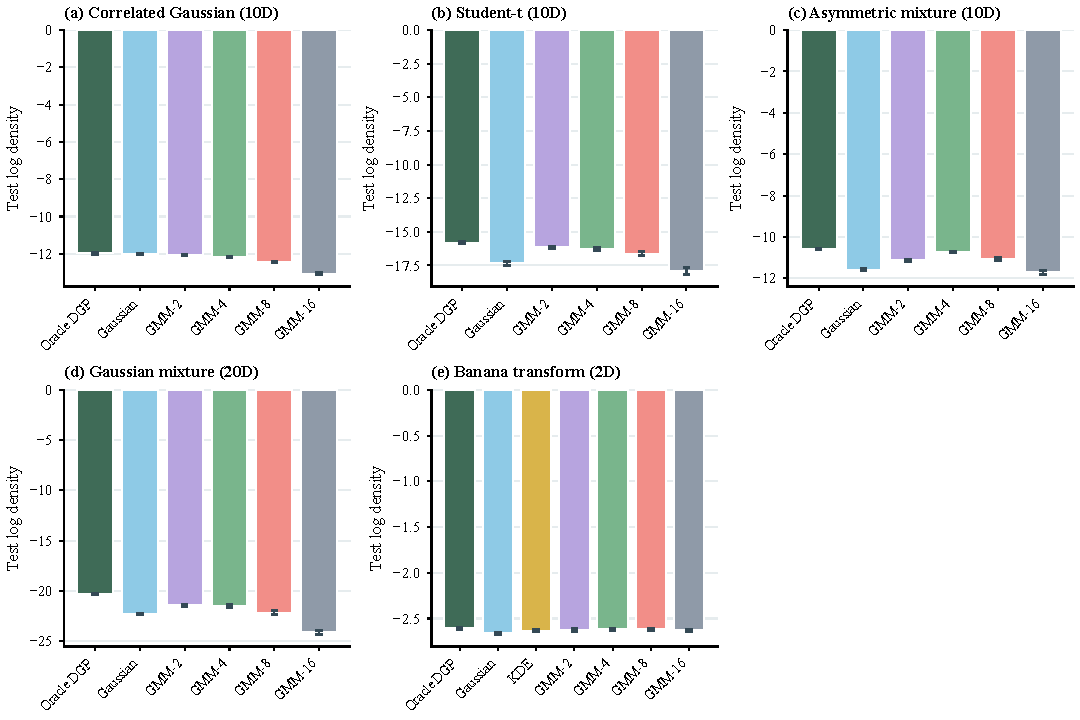
\includegraphics[width=\linewidth,clip]{figures/classical_density_controls.pdf}
\caption{Classical distributions: correlated Gaussian, Student-$t$,
asymmetric Gaussian mixture, Gaussian mixture and banana transform.
Bars show mean test log density and one Monte Carlo SE over five
repetitions. The oracle is the generating density; no SFD is fitted.}
\label{fig:classical-controls}
\end{figure}

\paragraph{Classical-family settings.}
The first three distributions have ten coordinates, the Gaussian mixture
has twenty, and the banana transform has two. GMM sizes are $2,4,8,16$,
with maximum 50 iterations, tolerance $10^{-5}$ and covariance
regularization $10^{-5}$. KDE is included only for the two-dimensional
scenario. The base seed is 20260624. These reduced-scale controls are
separate from the 25-repetition known-skeleton diagnostic.

\clearpage
\paragraph{Copula-family settings.}
The Gaussian and Student-$t$ copulas have ten coordinates; Clayton has five.
The Gaussian correlation is $0.55$. The Student-$t$ copula has correlation
$0.45$ and $4.5$ degrees of freedom. The Clayton parameter is $1.6$.
GMM sizes are $2,4,8,16$, with maximum 60 iterations, tolerance $10^{-5}$
and covariance regularization $10^{-5}$; KDE is included for Clayton only.
The base seed is 20260624. These controls do not include a fitted vine copula.

\begin{figure}[H]
\centering
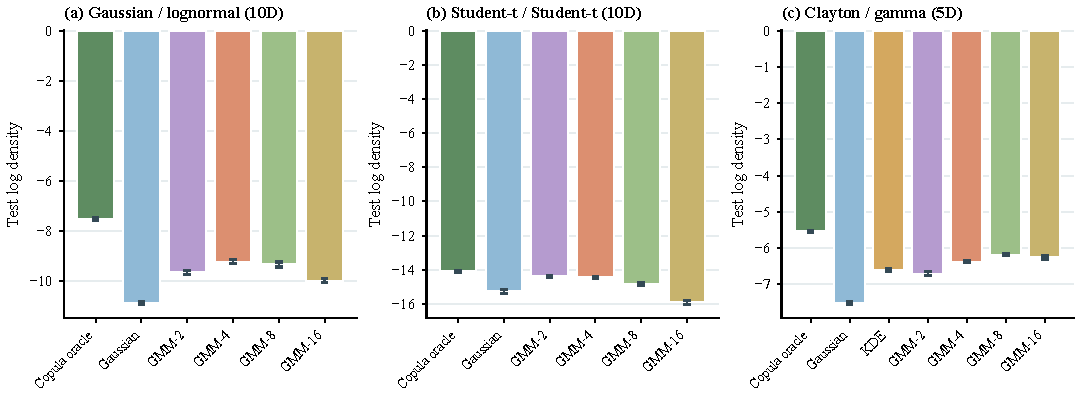
\includegraphics[width=\linewidth,clip]{figures/copula_density_controls.pdf}
\caption{Copula families: Gaussian with lognormal margins, Student-$t$
with Student-$t$ margins, and Clayton with gamma margins. Bars show mean
test log density and one Monte Carlo SE over five repetitions. The oracle
includes the copula and marginal densities; no SFD is fitted.}
\label{fig:copula-controls}
\end{figure}
\FloatBarrier


\end{document}
